\documentclass[a4paper,12pt]{article}
\usepackage[english]{babel}
\usepackage[utf8]{inputenc}

\usepackage[T1]{fontenc}
\usepackage{palatino}
\usepackage{amsfonts}
\usepackage{alicecwg}
\usepackage{array}
\usepackage{color}
\usepackage{lineno}
\usepackage{amssymb}
\usepackage{xspace}
\usepackage{booktabs}
\usepackage{textcomp}
\usepackage{multirow}
\usepackage{hyperref,url}

\alicecwg{6+7}
\version{1}
\title{Conceptual design note for calibration and reconstruction}

\author{
  <+author+>$^a$ \and <+author+>$^a$ \and <+author+>$^b$
}
\institutes{
  \normalsize{\it $^a$ <+Institute 1+>}\\
  \normalsize{\it $^b$ <+Institute 2+>}
}

\date{\today}

\newcommand{\TBD}        {\textcolor{red}}
\newcommand{\aliroot}    {\textit{aliroot}\xspace}
\newcommand{\row}        {\textit{row}\xspace}
\newcommand{\col}        {\textit{col}\xspace}
\newcommand{\TF}         {\textit{TF}\xspace}
\newcommand{\CI}         {\textit{CI}\xspace}
\newcommand{\TI}         {\textit{TI}\xspace}
\newcommand{\Tz}         {\ensuremath{t_{0}}\xspace}
\newcommand{\pp}         {pp\xspace}
\newcommand{\ee}         {{e$^+$e$^-$}\xspace}
\newcommand{\ppb}        {p--Pb\xspace}
\newcommand{\pbp}        {Pb--p\xspace}
\newcommand{\pbpb}       {Pb--Pb\xspace}
\newcommand{\auau}       {Au--Au\xspace}
\newcommand{\ums}        {\ensuremath{\mu s}\xspace}
\newcommand{\ms}         {\ensuremath{ms}\xspace}
\newcommand{\sqrts}      {\ensuremath{\sqrt{s}}\xspace}
\newcommand{\sqrtsnn}    {\ensuremath{\sqrt{s_\mathrm{NN}}}\xspace}
\newcommand{\gevc}       {~\ensuremath{\mathrm{GeV}\!/c}\xspace}
\newcommand{\mevc}       {~\ensuremath{\mathrm{MeV}\!/c}\xspace}
\newcommand{\lumi}       {\ensuremath{\mathcal{L}}\xspace}
\newcommand{\mum }       {~\ensuremath{\mu\mathrm{m}}\xspace}
 
%\newcommand{\oo}         {\ensuremath{O^2}\xspace}
\newcommand{\oo}         {O\ensuremath{^2}\xspace}


\newcommand{\pim}        {\ensuremath{\pi^-}\xspace}
\newcommand{\pip}        {\ensuremath{\pi^+}\xspace}
\newcommand{\pizero}     {\ensuremath{\pi^0}\xspace}
\newcommand{\kam}        {\ensuremath{K^-}\xspace}
\newcommand{\kap}        {\ensuremath{K^+}\xspace}
\newcommand{\kzerol}     {\ensuremath{K^0_L}\xspace}
\newcommand{\kzeros}     {\ensuremath{K^0_S}\xspace}
\newcommand{\jpsi}       {\ensuremath{\mathrm{J/}\psi}\xspace}

\newcommand{\pt}         {\ensuremath{p_\mathrm{T}}\xspace}
\newcommand{\meanpt}     {\ensuremath{\langle\pt\rangle}\xspace}
\newcommand{\mt}         {\ensuremath{m_\mathrm{T}}\xspace}
\newcommand{\Et}         {\ensuremath{E_\mathrm{T}}\xspace}

\newcommand{\nch}        {\ensuremath{N_\mathrm{ch}}\xspace}
\newcommand{\dndy}       {\ensuremath{\mathrm{d}\nch/\mathrm{d}y}\xspace}
\newcommand{\dndeta}     {\ensuremath{\mathrm{d}\nch/\mathrm{d}\eta}\xspace}
\newcommand{\meandndeta} {\ensuremath{\langle\dndeta\rangle}\xspace}
\newcommand{\ezdc}       {\ensuremath{E_\mathrm{ZDC}}\xspace}
\newcommand{\degr}       {\ensuremath{^\circ}\xspace}
\newcommand{\dens}       {charged-particle pseudorapidity density\xspace}
\newcommand{\npart}      {\ensuremath{N_\mathrm{part}}\xspace}
\newcommand{\ncol}       {\ensuremath{N_\mathrm{coll}}\xspace}
\newcommand{\dedx}       {\ensuremath{\mathrm{d}E/\mathrm{d}x}\xspace}
\newcommand{\vd}         {\ensuremath{v_\mathrm{drift}}\xspace}
\newcommand{\tz}         {\ensuremath{t_0}\xspace}

\newcommand{\0}          {\hphantom{0}} % for padding in tables

%% new commands for the jet chapter

\newcommand{\ptjet}{\ensuremath{\pt^{\rm jet}}\xspace}
\newcommand{\pthadron}{\ensuremath{\pt^{\rm hadron}}\xspace}
\newcommand{\rr}{\ensuremath{R}}

\newcommand{\Eclust}{\ensuremath{E_{\rm{clust}}}\xspace}
\newcommand{\sump}{\ensuremath{\Sigma_{\rm{p}}\xspace}}
\newcommand{\fsub}{\ensuremath{f_{\rm{sub}}}\xspace}

\newcommand{\Ecorr}{\ensuremath{E_{\rm{corr}}}\xspace}
\newcommand{\Ereco}{\ensuremath{E_{\rm{reco}}}\xspace}
\newcommand{\sumpt}{\ensuremath{\sum\left(p_{\rm matched}^{\rm track}\right)}\xspace}
\newcommand{\DEcorr}{\ensuremath{\Delta\Ecorr}\xspace}
\newcommand{\DEmc}{\ensuremath{\Delta{E_{\rm{MC}}}}\xspace}
\newcommand{\Rcorr}{\ensuremath{R_{\rm{corr}}\xspace}}

\newcommand{\ptcorr}{\ensuremath{\pt^{\rm corr}}\xspace}
\newcommand{\ptraw}{\ensuremath{\pt^{\rm raw}}\xspace}
\newcommand{\Ajet}{\ensuremath{A_{\rm jet}}\xspace}

%% Luminosity units

\newcommand{\invmb}{\mathrm{mb}^{-1}}      % /mb
\newcommand{\invmbps}{\invmb\mathrm{s}^{-1}} % /mb/s

\newcommand{\invub}{\mu\mathrm{b}^{-1}}      % /ub
\newcommand{\invubps}{\invub\mathrm{s}^{-1}} % /ub/s

\newcommand{\invnb}{\mathrm{nb}^{-1}}        % /nb
\newcommand{\invnbps}{\invnb\mathrm{s}^{-1}} % /nb/s

\newcommand{\invpb}{\mathrm{pb}^{-1}}        % /pb
\newcommand{\invpbps}{\invpb\mathrm{s}^{-1}} % /pb/s

%

\newcommand{\Minbias}{Minimum bias\xspace}
\newcommand{\minbias}{minimum bias\xspace}

\newcommand{\fee}{front-end electronics\xspace}

\newcommand{\run}[1]{\textsc{Run\,#1}}

\newcommand{\figref}[1]{Fig.~\ref{#1}}
\newcommand{\Figref}[1]{Figure~\ref{#1}}
%
\newcommand{\tabref}[1]{Tab.~\ref{#1}}
\newcommand{\Tabref}[1]{Table~\ref{#1}}
%
\newcommand{\appref}[1]{appendix~\ref{#1}}
\newcommand{\Appref}[1]{Appendix~\ref{#1}}
%
\newcommand{\secs}{Secs.\xspace}
\newcommand{\Secs}{Sections\xspace}
\newcommand{\secref}[1]{Sec.~\ref{#1}}
\newcommand{\Secref}[1]{Section~\ref{#1}}
%
\newcommand{\chaps}{Chaps.\xspace}
\newcommand{\Chaps}{Chapters\xspace}
\newcommand{\chapref}[1]{Chap.~\ref{#1}}
\newcommand{\Chapref}[1]{Chapter~\ref{#1}}


\begin{document}
\maketitle

\linenumbers

\begin{abstract}
This note defines the goals of the calibration and reconstruction in
ALICE \oo project and outlines the procedures need to achieve these goals.
We summarize the current understanding of data rates from detectors on
different stages of processing...
\end{abstract}
\newpage

\begin{changelog}
  \change{1}{08/12/13}{
    initial version on alice-o2-cwg7/doc/cwg67cdn
    git clone https://git.cern.ch/reps/alice-o2-cwg7
  }
\end{changelog}

\tableofcontents

\newpage

%-------------------------------------------------------
\section{Introduction}
The reconstruction and calibration can be loosely split in two phases:

\begin{itemize}

\item Online: performed during the data taking on the data received from the
upstream components of the processing chain or short time buffers.
While the primary aim of these operations is to achieve a data
compression level acceptable for the permanent storage at \TBD{$\sim$12.4
GB/s in average and $\sim$75 GB/s peak rate}~\cite{panelDoc}, they
should also
facilitate as much as possible further processing of data to analysis
grade level. 
The calibrations performed at this phase should minimize
the loss of the useful data during the lossy compression steps and
preferably allow later reconstruction for physics analysis without
special calibration passes.

\item Offline: decoupled from the data taking process, using as an input the
data from the permanent storage. Its aim is to provide analysis grade
level for the full detector, analyzable in terms of separate
collisions.
\end{itemize}

The online reconstruction and calibration proceed in two phases on:

\begin{itemize}
\item First Level Processors (FLP), receiving raw data from the
Detector Data Links (DDL). Each FLP sees all data (e.g. all
time-slices, without omissions)
from only the part of detector it services. The data from FLP's are 
aggregated and split into pieces containing information from all detectors for
predefined time-frames (\TF).
\item Event Processing Nodes (EPN), which process \TF's
  asynchronously.
\end{itemize}



%-------------------------------------------------------
\section{Reconstruction and calibration flow}
\TBD{This section gives general description of reconstruction and
  calibration:
\begin{itemize}
\item Definitions of Calibration Interval (\CI) and Update Interval (\TI)
\item State why kind of data is calibrated/reconstructed in FLP's
  (clusters, masks ets) and what on EPNs
\item How the calibration from FLP propagates to EPNs and from FLP and
  EPN's to OCDB. 
\item Treatment of \TF edges in calibration and reconstruction
\item Preferences for the \TF duration (variable, fixed)
\item Calibration feedback loop ("predictive step").
\item Outline of reconstruction flow, detector dependencies.
\item Alternatives: full reconstruction at once vs partial
  reconstruction (e.g. high \pt tracks) for calibration ("cpass") followed by
  full reconstruction.
\end{itemize}
}

One of the main challenges for ALICE at \run{3} is without doubt the extremely high data taking rates that will 
bring the experiment to receive data with a speed 2 orders of magnitude higher than at \run{1}, 
jumping from 500 Hz to 50 kHz. The physics motivations for this were well described in~\ref{upgradeLOI}. Here,
the necessity to perform online calibration and reconstruction was also presented, with the main aim at 
reducing the data volume to an affordable size for permanent storage. 

The highest data reduction factor which
is expected is $\sim 20$, coming from the TPC detector which will be read out in continuous mode at \run{3} leading
otherwise to unaffordable data storage.
It is clear that to achieve such factors, zero suppression techniques and coding algorithms won't be enough, and 
a substantial part of the data reduction will be reached only through reconstruction of tracks discarding the data
that do not carry physics information (e.g. clusters from
$\delta$-rays, unreconstructable tracks etc.). 

The strong coupling between calibration and reconstruction that was effectively demonstrated during \run{1} will 
be complicated by the extreme conditions in terms of luminosity that will characterize \run{3} data taking. Time
dependence of calibration will become even more pronounced, and the statistics requirements of calibration 
will have to deal with the new data flow that will accommodate both continuous and triggered read out.  

In order to understand the calibration and reconstruction data flow, it is important to summarize a few concepts.
\begin{itemize}
	\item \textit{Time Frame (TF)}: data will be sent from the FLPs to the EPNs after being aggregated in blocks where multiple
	events will be present at the same time, in order to combine the data from detectors read in triggered and 
	continuous mode; the boundaries of the time frames will be defined by a heartbeat triggered received by all detectors. The
	foreseen duration of the TF will be $\sim 100$ times the drift time inside the TPC detector. The possibility to 
	have an adjustable TF duration which counterbalance the decrease in luminosity in time in order to level the 
	statistics contained in one TF is under discussion. Both scenarios (namely, fixed and varying TF duration) have to 
	be considered when defining the calibration and reconstruction data flow.
	\item \textit{Calibration Interval (CI)}: \textcolor{red}{I am not sure whether this is important...} since calibration is strongly
	related to the data taking conditions, a CI can be defined as a period where stability is guaranteed. This could refer 
	to detector configuration, beam conditions... 
	\item \textit{Update Interval (UI)}: time-dependent calibrations require an update of the relevant calibration parameters
	with a frequency that strongly depends on the calibration itself (and as such, on the detector and its requirements). A UI 
	corresponds to the time between the moment when calibration data start to be collected, and the last moment when they
	are used. In terms of data taking this corresponds to a period during which a detector can be considered stable. 
	\item \textit{Feedback Loop (FL)}: the interdependency of calibration and reconstruction that was fully demonstrated during 
	\run{1} implies that calibrations that are produced during reconstruction should be then used for the reconstruction 
	of the next data. The FL is the concepts that describes this dependency.
\end{itemize} 

\subsection{Processing in FLPs}
\label{sec:Processing in FLPs}
The first layer of data processing will be the FLP. Here, the data will come from the detectors through DDL links and 
RORC3 cards. RORC3 cards will be equipped \textcolor{red}{(I guess)} with FPGA cards, where cluster finding will be 
possible as it was done during \run{1} for the TPC. When shipped to the FLPs' memory, further data processing will 
be possible, exploiting possible GPUs on 
the machines. The single FLP is foreseen to be connected to a maximum
of 12 optical links, while for instance, the TPC will be served by
1836 DDLs.
. \textcolor{red}{It is not
clear to me whether, in case a detector has only one DDL, it will be connected to the same FLP as another detector, but
I assume not. In any case, I don't foreseen any cross-talk between
different detector's data.}. 
This, obviously, limits the amount of 
data that can be processed in an FLP per detector, and as a consequence rules out at this stage any processing that
relies on the whole detector's data and/or on data from different detectors. Procedures such as cluster finding will 
be limited to the part of detector connected to the FLP. As a result, the same physical cluster could be found on two 
different FLPs. The way this doubled information will be treated in the EPNs will be detector specific, and could imply
merging of clusters, or discarding of one of the two. 

It is important to mention here that FLPs will receive all the data from the detector part they are connected to. Despite the
limit in ``detector slice'' it is processing that it
% will occur at this stage 
will 
%then 
benefit from having at its disposal all the statistics. 

As already mentioned, data will come to the detectors with a rate of 50 kHz, with a peak input to the FLPs of 1 TByte/s. 
Assuming 250 FLPs in the online farm (following the current estimates from the O$^2$ project), each FLP will receive
4 GByte/s. With a tentative hypothesis of 20 GBytes of memory in each FLP dedicated to data processing, and bearing in 
mind that part of the resources will be used for data transport, one could conclude that a processing rate of 2 s/GByte
could be reasonable. Nevertheless, the data will have to be exported to the second layer of processing with the same 
frequency with which they arrived on the FLPs, in order to not create data traffic jam over the network. 

\subsection{Processing in EPNs}
\label{sec:Processing in EPNs}
From the FLPs, data are aggregated in time frames, and then sent to EPNs. The length of a TF will be of the order of
$100 \div 1000$ times the drift time in the volume of the TPC ($\sim 100 \mu s$), which means $10 \div 100$ ms. Whether such
duration will be fixed or variable is currently under discussion. For simplicity we will assume here that it is fixed to 
$100$ ms. 

While on the FLPs data are split per detector and per detector ``slices', on the EPNs they will be merged together. 
This is an important difference with respect to EPNs, since interconnections between detectors will be possible at this 
stage. On top of containing the data read-out by the detectors, the TF will also transport from the FLPs the calibration
information that was produced there (if any, and as soon as they are available). Due to the processing rate of the FLPs,
and to possible statistics requirements for calibrations, it could happen that some calibrations are ready to be sent 
the the EPNs only after a certain amount of time frames have been collected and prepared. \textcolor{red}{It is to be evaluated 
whether such cases exist, how much statistics they would need, and then one should combine it with the possibility
that TF are sent not one-by-one, but in groups of many (as presented at the O$^2$ meeting in January). If the second
option is implemented, maybe there is time to prepare the calibrations before sending the data to EPNs.} The calibration
data size is expected to be smaller and negligible compared to the detector data size.

On top of receiving the data from the detectors, the EPNs will also 
receive data from
%be connected to 
the Detector Control System (DCS
\textcolor{red}{at least I hope}), which will add to the time frame \textcolor{red}{(I don't know if embedded
in the data or not)} detector specific information such as configurations, temperatures and high voltages. The DCS 
information could be used as input for calibrations in the EPNs. 

The EPNs will be the natural place to perform the first steps of the 
%reconstruction
tracking. Due to the fact that only a course
calibration is possible at this stage, the primary goal of this reconstruction should be data reduction. For this reason, 
mainly detector standalone procedures are expected to occur at this stage, such as ITS track finding and fitting, 
vertexing, TPC track finding, and only limited to those steps for which a first level calibration is enough. 

In case tracking is needed for the calibrations to be used at this point, it is important to bear in mind that the data flow in 
terms of time frames imposes some limitations, together with the fact that each EPN is independent from the 
others, and that no information can be exchanged (at this stage) between the EPNs. The distribution of the TF over 
the different EPNs in ``round-robin'', for example, implies that each
EPN will receive (in average) a second time frame only after a 
time equal to the duration of a time frame multiplied by the number of EPNs, i.e., assuming 1500 EPNs, and a TF duration 
of 100 ms, after 2.5 minutes. If some calibrations should occur in the EPNs needing a statistics that can be collected over a 
time which is of the same order as the TF duration, they will then be available only for the subsequent time frame. This 
is possible only if the UI of a calibration is long enough to ensure the stability of the calibration over this time. Even more
complicated is the case when more than one TF is needed to collect the statistics for calibration. The time to be waited
before a calibration can be used would then stretch over several minutes. It is necessary to evaluate which calibration
procedures needed at this first reconstruction step would be affected by this. 

On the other hand, calibrations that take as input only a very limited amount of data collected over a time which is much
smaller than the TF duration could be produced with the first data of the TF, and then used in the reconstruction of the
remaining portion of TF. Depending on the validity of such calibrations, it could be that as soon as a calibration object 
is produced, it is used over several TFs on the same EPN. 

Due to the fact that the EPNs receive the data from all detectors corresponding to the same time frame, in case the 
calibration of one detector depends on the reconstructed data of another one, the reconstruction flow will have to 
follow this requirement \textcolor{red}{(an example is TPC that needs event and track multiplicity information from FIT)}.
Never the less, whenever the calibration of one detector (let's say detector B) depends on the calibration of another
(let's say detector A), a more sophisticated
procedure will have to be adopted. In the assumption that no circular dependency is there between two detectors, 
and that both detectors need to calibrate a fraction of data that is much smaller that the TF duration, one possible 
solution is to start reconstructing, produce with the first data the calibration of detector A, make it available for 
the reconstruction of the rest of the data, and produce the calibration for detector B. This approach implies the 
possibility to produce and use a calibration during the reconstruction of the same TF. An analogous implementation
could be realized in case for the calibration of detector A and B a whole TF is needed, baring in mind the delay
between two TFs on the same EPNs. These considerations make it clear the importance of determining 
inter-detector dependencies.

\subsection{Processing after data reduction}
\label{sec:Processing after data reduction}
In the following, the data flow will be split into steps, as shown in Figure~\ref{fig:Flow}. 

\subsubsection{Step 1}
\label{sec:Step 1}
As it was already discussed, 
clusterization and first 
calibrations are supposed to happen at the beginning of the processing. As soon as the data are assembled in 
one time frame, this is shipped to one EPN. Here, the first algorithms that will be run will be most likely standalone
procedures aimed at data reduction. EPNs should also be able to receive data from DCS. To be noted that at the
very beginning of the fill only the calibrations from the previous fill will be available. As a consequence, in case the 
standalone processing will need calibration from FLPs, either some delay is introduced between FLPs and EPNs
in order to prepare such calibrations, or the first data shipped to the EPNs will not be processed here with the most 
recent calibrations. In the latter case, it could be envisaged, though, a second processing of these data to recover 
them.

The calibrations that are produced at this stage of the processing will be available during the same stage only for the 
data that will come to the same EPNs. This means that up to data compression no cross-talk is foreseen between the
different EPNs. This should be possible since up to this moment no calibrations requiring large fraction of the statistics
seem to be needed. Never the less, EPNs should be able to read from an OCDB-equivalent calibration database 
in order to make use of the calibrations produced in previously standalone runs (e.g. PEDESTAL, NOISE... runs). The 
drawback of such approach is that in case data compression requires some calibrations from the standalone reconstructions,
the first portion of data on each EPN will not be calibrated at first, and a second processing over them will be needed
to recuperate them. The feasibility of such implementation depends on the same argumentations mentioned in 
Sec.~\ref{sec:Processing in EPNs} concerning calibration validity. 

\begin{figure}[htp!]
  \begin{center}
    \includegraphics[height=0.67\textheight, angle =90]{general/flow_scenarios.pdf}
    \caption{Schematic
      outline of the reconstruction and calibration data flow.}
    \label{fig:Flow}
  \end{center}
\end{figure}

\subsubsection{Step 2}
\label{sec:Step 2}
The data flow continues from this point with the first inter-detector matching, and tracking stages that could not be performed
before due to missing calibrations. 
% RS: supress?
These processes would still happen on time frame base, on the EPNs. 
%
For example, a first ITS-TPC matching could be performed, and the TRD tracking seeding
using TPC information could take place. \textcolor{red}{Supposing that the TPC output from the EPN is at this point
calibrated enough, TRD could perform its own calibration using tracks, so they would need to match with TPC. For the 
TRD calibration, the same argumentations as in Sec.~\ref{sec:Processing in EPNs} in order to obtain and use the
calibration information on the EPNs.
Moreover, at this step,
a high and low \pt sample could be extracted from the ITS-TPC (also TRD?) matching to provide the rescaling factor 
for the Space-Charge Monte Carlo reference map to be adjusted to the current data taking. Independently from where 
everything is happening online or offline after data reduction, such sample could be prepared online anyway. At this point,
thanks to the fact that the rescaling of the reference map is needed with a frequency of $\sim 10$ mins, 
there are two possibilities:
\begin{enumerate}
	\item a subset (one or more) of EPNs is dedicated to the ITS-TPC matching; as such, they should prepare the rescaling
	factor to be then propagated back (through an OCDB server?) to all EPNs (including themselves) to perform standalone 
	reconstruction for data reduction; this would have the advantage of a single object used in all EPNs; the usage of a limited number
	of EPNs would probably reduce the time necessary to prepare the calibration;
	\item each EPN collects the ITS-TPC matching sample to rescale the reference map when processing the data that the 
	EPN itself will receive; this would have the advantage of decreasing the amount of data to be exchanged, with the drawback
	to have to take into account various objects for different time frames that reach different EPNs in a non-predetermined order.
\end{enumerate}
}  

\subsubsection{Step 3}
\label{sec:Step 3}
Step 3 should be dedicated to the final calibration processes for the tracking detectors \textcolor{red}{mainly
the TPC and TRD (obviously, if TRD gets calibrated here, TPC will match with it when it is still not fully calibrated}. Again, being 
on the EPNs, the same argumentations as inSec.~\ref{sec:Processing in EPNs} in terms of statistics and validity apply. To this step
also a final ITS-TPC-TRD matching should belong, together with a refit of the tracks profiting from the updated calibrations.

\subsubsection{Step 4}
\label{sec:Step 4}
The last step of the data flow would include matching with the outer detectors, calibrations that require the best barrel tracking 
performance and in particular those to provide PID information, V0 reconstruction, and, finally, event building. The output of step 
4 would be physics-grade data. 

\subsection{Processing partitioning: online, quasi-online, offline}
\label{sec:Processing partitioning: online, quasi-online, offline}
After data reduction has been achieved to the level required by data storage, two main possible extreme scenarios could 
be envisaged in terms of ''processing partitioning``, i.e. the moment, with respect to data taking, when the different steps
described in~\ref{sec:Processing after data reduction} take place.
 
In the first case, the reconstruction and calibration processes continue in online mode on the O$^2$ farm to deliver
as final output physics-level data. This could be possible only in case the different stages of the subsequent 
reconstruction and calibration could be completed with the final performance by the beginning of the subsequent
fill. In the second case, only compressed data are foreseen to be stored by the beginning of the next fill, and all 
the remaining reconstruction and calibration will be processed in quasi-online or even offline mode. 

CPU timing, memory, and inter-detector dependencies will determine which of the two option, or an intermediate
scenario between the two, will be feasible. One requirement is nonetheless that the final output for physics should be
reproduced starting from the compressed data and the calibrations at any time, allowing also for further improvements 
in the output itself. 

One possibility could be to restrict to online only step 1 including part of step 2, namely the ITS-TPC reconstruction 
of high/low \pt tracks to allow for the creation of the average TPC space charge map out of the reference one from
Monte Carlo. This reconstruction part could occur on a dedicated, small portion of EPNs, while the bulk of the farm
is dedicated to run the remaining steps. 

Due to the fact that MUON data might not depend on the other detectors, they could be processed asynchronously after step 1.

An alternative to storing compressed data and then AOD-like data is to add an intermediate storage phase at the end
of step 3 with tracks built in ITS-TPC-TRD (the main detectors needed for TPC calibration), with the data from the 
outer detectors, so that the matching to them could be repeated without needing to reprocess also step 2.
 

\subsection{Possible data flow implementation}
  






















%-------------------------------------------------------
\section{Handling of continuous readout}

\TBD{
Describe how the processing of data from detectors with continuous
readout is done.
\begin{itemize}
\item ITS: treatment of collisions split between two read-out cycles
\item TPC: reconstruction with seeds corresponding to specific \Tz
  (from FIT) vs simultaneous reconstruction of multiple \Tz's (from
  FIT or in standalone mode)
\item ...
\end{itemize}
}

%-------------------------------------------------------
\section{Data rates and constraints}

\TBD{This section summarized current estimates on raw data rates normalized
to \pbpb 50 kHz interaction rates.}
\TBD{Give min/max limits for those detectors whose rate is still uncertain.}

\begin{table}[ht]
\begin{tabular}{ |l|l|l|l| } \hline
Detector & Input to FLP's & Input to EPNs & average storage rate \\ \hline
TPC & 1 TB/s                                 & xxx & xxx \\ \hline
TRD & \begin{tabular}{@{}l@{}} 10-20 GB/s (tracklets)\\ 18 GB/s (partial raw)\end{tabular} & xxx & xxx \\ \hline
ITS & \begin{tabular}{@{}l@{}} 30 GB/s with noise\\ 8.2 GB/s w/o noise\end{tabular} & xxx & xxx \\ \hline
ZDC & \begin{tabular}{@{}l@{}} 30 MB/s (Min.Bias)\\ 160 MB/s (self-triggered)\end{tabular} & xxx & xxx \\ \hline
MUON & 1.5 GB/s                              & 1.2 GB/s & \begin{tabular}{@{}l@{}}9 - 400 MB/s\\see \ref{MUON:EPN} for details\end{tabular} \\ \hline
FIT & 115 MB/s                               & xxx & xxx \\ \hline
TOF & 1.8 GB/s & 1.4 GB/s & 1.4 GB/s \\ \hline
... & ...                                    & xxx & xxx \\ \hline
\end{tabular}
\caption{
\TBD{Summary of expected data rates at different stages of processing 
for \pbpb hadronic interaction rate of 50 kHz.}
}
\label{tab:InputRate}
\end{table}


\subsection{TRD}
\label{TRD:datarate}

For Run-3 the TRD will have to be adapted to the higher interaction
rates by modifying the FEE and readout system.  The chosen strategy is
based on using the existing FEE in a different mode of operation which
limits the amount of event data to be read.  The currently employed
mode of reading full zero-suppressed ADC data results in readout times
of several 10~$\mu$s, which will be too long for Run-3 conditions.
Therefore the following alternatives are foreseen:
\begin{itemize}
\item {\bf Tracklet Readout} In this mode only the information on the
  online tracklets is transferred, thus avoiding the handshaking
  overhead in the raw readout mode and allowing event readout times
  between 4~-~8~$\mu$s.
\item {\bf Partial Data Readout} The readout of the full raw ADC data
  would in this mode be limited to regions where TRD information is
  relevant (i.e. where tracklets fulfilling simple criteria for
  electron candidates).
\item {\bf Mixed Mode} If necessary, e.g. for calibration purposes,
  also a mixed mode can be foreseen.  This means that only for a very
  small fraction of events (e.g. $10^{-3}$) the full zero-suppressed
  raw ADC data is transferred, while the rest of the events is read in
  one of the two reduced readout modes (tracklet readout or partial
  data readout).
\end{itemize}
%
The expected data rates are summarized for the first two options in
Tab.~\ref{tab:TRD:eventSize}.  For the mixed mode option no
significant change of the data rate is to be expected, if the fraction
of events with full readout is kept at a small enough level.
%
\begin{table}[ht]
  \centering
  \begin{tabular}{|c|c|c|}\hline
    Readout mode         & Interaction rate (kHz) & Data volume (Gbit/s/sector) \\ \hline
    Tracklet readout     & 50                     & 4.73 - 8.78    \\
                         & 100                    & 7.68 - 13.65   \\ \hline
    Partial Data Readout & 50                     & 7.8            \\ \hline
  \end{tabular}
  \caption{Estimated data rate for Pb-Pb collisions for the TRD
    detector.}
  \label{tab:TRD:eventSize}
\end{table}

\subsection{ITS}
\label{ITS:datarate}

Table~\ref{tab:ITSrate} summarizes the hit rate in the ITS expected in continuous readout with
30\ums frames at 50kHz \pbpb collisions, including the contribution from the QED electrons and 
random noise at the rate of $10^{-5}$ per pixel in $2.5\times 10^{10}$ channels. 
Minimum bias collision multiplicity is assumed to be 1/3 of that in
the central collision

\begin{table}[ht]
\begin{tabular}{ | p{0.8cm} | p{1.6cm} | p{1.6cm} | p{1.8cm} | p{2cm} | p{3cm} | }
%\begin{tabular}{ | l | l | l | l | l | l | }
\hline
   & \multicolumn{3}{|c|}{Single central \pbpb collision} & QED 30 \ums @ 50kHz & Min.bias \pbpb 30 \ums @ 50kHz \\ \hline
Lr & Min per sensor & Max per sensor & Mean per layer & Mean per layer      & Mean per layer        \\ \hline
0  & 31             & 137            & 9948           & 8400                & 13400                 \\ \hline
1  & 30             & 92             & 9468           & 5400                & 10100                 \\ \hline
2  & 26             & 67             & 8978           & 3400                &  7900                 \\ \hline
3  & 1.7            & 4.7            & 8732           & 120                 &  4500                 \\ \hline
4  & 1.4            & 3.0            & 7717           & 72                  &  3900                 \\ \hline
5  & 0.62           & 1.55           & 9336           & 52                  &  4700                 \\ \hline
6  & 0.55           & 1.22           & 8819           & 44                  &  4500                 \\ \hline
\multicolumn{5}{|c|}{Total hit clusters per 30 \ums frame}                  & 49000                 \\ \hline
\multicolumn{5}{|c|}{Noisy pixels in 2.5$\times 10^{10}$ channels}          & 250000                \\ \hline
\hline
\end{tabular}
\caption{Hit rates from hadronic collisions and QED electrons. Random noise rate assumed to be $10^{-5}$ per pixel per 30\ums 
readout frame.}
\label{tab:ITSrate}
\end{table}

As one can see, the data rate is dominated by the noise, which
produces only single-pixel clusters. According to simulations,
the single-pixel cluster probability from real hits is $\sim 1.2\%$, 
and $\sim 70\%$ of such pixels are in fact split from larger
clusters produced by the same particle. Therefore, one can consider
discarding single-pixel clusters either in the FE or during the
clusterization on the FLPs. But, given that the detector design is not
final yet, the fraction of real single-pixel clusters may 
increase (particularly, for larger pixel pitch). For the conservative estimate of ITS data rate on the 
input to the online system we assume that the single-pixel clusters (if
not suppressed) will be packed using 20 bits per cluster while
remaining hits will consume in average 40 bits per clusters (by
storing the row, column and 4$\times$4 pixels plaquette (partially)
containing the cluster. This leads to $\sim$ 30 (8.2) GB/s at 50~kHz and
$\sim$ 38 (16.4) GB/s at 100~kHz without (with) suppression of the single-pixel
clusters.

\subsection{ZDC}
\label{ZDC:datarate}

The ZDC will be triggered either by the ALICE minimum bias trigger or auto-triggered and no continuos readout is foreseen.
The expected data rates for Pb-Pb collisions at 50 kHz are $\sim$30~Mb/s with the ALICE minimum bias trigger (without dead time) and $\sim$160~Mb/s when triggering with the ZDC (there is a factor 25 in the expected rate that derives from ratio of electromagnetic dissociation cross section and the hadronic cross section but in this case we add a dead time due to the VME).

For Run III the ZDC QDCs will be replaced by digitizers with 12 bit, 1~Gs/s sampling frequency and on-board FPGAs that allow fast pre-processing of data. In particular the baseline is measured and its contribution is directly subtracted from the signal. The payload reduced to 3 words for each channel (namely the integral and the time arrival of the signal with high and coarse resolution) with an estimated payload 
of $\sim$600~b per event, therefore no further compression is foreseen. 

\subsection{PHOS}
\label{PHOS:datarate}

During Run-3, PHOS will take triggered data, like in Run-1 and
Run-2. Raw data format and event size will not change in Run-3, it
will be digitized 10-bit amplitudes sampled at a rate 10~MHz by the
ALTRO chip. Each amplitude is measured by two ADC channels, delivered
from two preamplifiers with high and low gains. The number of samples
is configurable. A reduction of the number of samples without
degradation of the amplitude and timing accuracy is planned for
Run-3. Redundancy of the amplitude measurement by two channels with
high and low gain can also be eliminated. Thus, that the average event
size in Run-3 will reduce by a factor of $2-3$ compared with
Run-1. Table~\ref{tab:PHOS:eventSize} summarizes event size in PHOS
per one DDL link and for the whole detector in pp, p-Pb and Pb-Pb
runs.
%
\begin{table}[ht]
  \centering
  \begin{tabular}{|c|c|c|c|}\hline
    System              & pp     & p-Pb   & Pb-Pb \\ \hline
    Event size per DDL  & 0.5~kB & 0.8~kB & 1.4~kB \\
    Event size per PHOS & 14 kB  & 20 kB  & 40 kB \\ \hline
  \end{tabular}
  \caption{Estimated event size from the PHOS detector}
  \label{tab:PHOS:eventSize}
\end{table}
%
Given collision rate in Pb-Pb runs of 50~kHz, one expects to have a
data taking rate from PHOS to be 2~GB/s.

\subsection{MUON}
\label{MUON:datarate}

Data rate estimates for MUON are based on past observations from 
Run1 \pbpb runs. Even though we expect an increase in particle 
multiplicities (by $\sim$ 25\%), we know that the Muon Tracker (MCH) 
data size is to a large extent dominated by FEE noise, and 
that Muon Trigger (MTR currently that will become the MID, 
Muon Identifier) data size is a constant.  
As we expect that the new Muon Tracker FEE will solve the 
stability problems, we then assume that Run1 data 
sizes are a very reasonable estimate of Run3 data sizes. 
The Run1 data was heavily biased towards central events 
due to the trigger used, so the average event size was 
biased towards high values (60 kB/event for MCH). A more 
detailed analysis reveals that MB events are around 
25 kB/event and central ones around 75 kB/event. 
MID events are expected to be 3 kB/event (compared to the 
current 7 kB/event). So all in all the expected Muon data 
rate is $\sim$ 1.5 GB/s for 50~kHz MB.

Note that the upgrade of the MCH readout itself is actually 
designed to handle a much higher data rate\cite{Run3OnlineTDR}, 
as it must accept peak rates. Those have been estimated 
to 100 GB/s at 50~kHz, assuming peak occupancies of 9\% and a 
readout mode where all the ADC samples (10 of them per pad) are 
readout, for a total of 140 bits per pad. That mode of operation is to 
be considered a debug mode and will not be used in a sustained way. 
The normal, routine, readout mode will have only one charge and address 
per channel which amount to 90 bits per channel (per the SAMPA specification). 
We assume at this stage that it will be possible to reduce this (in the CRU, for instance) 
to 64 bits per channel.

\subsection{MFT}
\label{MFT:datarate}

The MFT is a Silicon tracker which will be installed in the muon spectrometer acceptance. It is composed of 6 planes of Silicon pixel sensors. A version with 5 planes was considered in the LoI Addendum. It has been decided to add a sixth plane for redundancy in the tracking. 
A description of the detector can be found in the ALICE LoI addendum~\cite{LOI_Addendum}.
In order to cover the full area, 668 ladders of 1 to 5 sensors with a total of 2530 sensors are necessary.

Three main components are contributing to the hit rate of the MFT: the Pb--Pb collision itself, the hits induced by the QED processes (mainly low $p_{T}$ electrons at low angles) and the noisy pixels.

Table~\ref{tab:MFTrate} summarizes the number of hits  in the MFT expected in the following conditions: continuous readout with
16~\ums frames at 100~kHz \pbpb collisions and 
a random noise at the rate of $10^{-5}$ per pixel. Minimum bias collision multiplicity is assumed to be one third of that in the central collision.


\begin{table}[ht]
\centering
\begin{tabular}{ | c | c | c | c | c |}
%\begin{tabular}{ | l | l | l | l | l | l | }
\hline
\multirow{2}{*}{Plane}   & Single central  & Min.bias \pbpb  &  QED & \multirow{2}{*}{Noisy Pixels} \\ 
    &  \pbpb collision &  16 \ums @ 100 kHz &  16 \ums @ 100 kHz & \\ \hline
0   & 3480           & 3016                & 1424     &     763       \\ \hline
1   & 3480           & 3016                & 1424     &      763      \\ \hline
2  & 3950           & 3423                & 1512      &       926    \\ \hline
3  & 3910           & 3389                &  1403       &      1090    \\ \hline
4  & 3820           & 3311                 &  1274        &      1205   \\ \hline
5  & 4100           & 3553                  &  1271         &     1325   \\ \hline
\multicolumn{2}{|c|}{Total hit clusters }                  & \multirow{2}{*}{19708}     &   \multirow{2}{*}{8308}     &   \multirow{2}{*}{6072}       \\ 
\multicolumn{2}{|c|}{per 16 \ums frame}                  &     &     &       \\ \hline
\end{tabular}
\caption{Hit rates from hadronic collisions and QED electrons. Random noise rate assumed to be $10^{-5}$ per pixel per 16~\ums 
readout frame.}
\label{tab:MFTrate}
\end{table}

Two kinds of clusters can be distinguished: single-pixel clusters which the primary source is noisy pixel and the multi-pixel clusters induced by particle crossing the detector. 
The clusters are assumed to be encoded into 40 bits per cluster.
The total data flow output is then estimated to be 10.1~GB/s for the entire MFT.
The data rate reduces to 7.2~GB/s when assuming a 50~kHz minimum bais \pbpb collision rate still with a 16~\ums readout time per frame.
With such raw data flow rate, an online clusterization is mandatory to reduce the amount of data written on tape (see section~\ref{sec:MFTClusterization}).

The local on-detector readout is proposed to be performed by GigaBit Transceiver (GBT) versatile link developed at CERN which will act as a data concentrator.
Fig.~\ref{fig:mft:schematic} presents a schematic of the readout scheme.
A total of 166 GBT links are foreseen to  handle the data flow.

\begin{figure}[h]
\centering
\includegraphics[width=0.9\textwidth]{MFT/Schematic.pdf}
\caption{\label{fig:mft:schematic} 
Possible schematic of the on-detector readout of the MFT using GBT as a concentrator.}
\end{figure}


\subsection{HMPID}
\label{HMPID:datarate}

No upgrade of the electronics is planned for HMPID. After the ALICE upgrade the HMPID will be able to exploit its maximum event read out rate
of 2.5 kHz in PbPb collisions, with an increasing factor of 4 w.r.t. Run 1 and Run
2 periods, when the drift time and the TPCread-out rate imposed lower rates. It will be triggered by a down-scaled ALICE minimum bias trigger.
Assuming that in minimum bias Pb-Pb collsions the chamber occupancy is $\approx$ 1\%, the expeced data rate per ddl will be $\approx$ 4 MB/s. 
HMPID has in total 14 ddls (2 per chamber). 



%-------------------------------------------------------
\section{Calibration, reconstruction and data reduction on FLP's}
\TBD{This section describes for each detector 
\begin{itemize}
\item What is done on the FLP, description of algorithms (if any)
\item Estimates on the processing rate
\item Estimates on the data rate sent to EPN's
\end{itemize}
}

\subsection{TRD calibration and reconstruction}
\label{TRD:FLP}

%-----------------------------------------------------------------------------
\subsubsection{Reconstruction}

The TRD reconstruction will have to follow different schemas,
depending on which type of readout is employed.  

In the case of the full raw ADC data readout or the partial data
readout, the it will follow essentially the same sequence as has been
used up to now.  It starts with cluster finding based on the raw data
for all read time bins, followed by the offline tracklet finding
(layer-by-layer).  This tracklet information is then the basis of the
global track finding using the Kalman filter.  For Run-3 the first two
steps (cluster and tracklet finding) might be run of the FLP, while
the track finding will be part of the EPN stage.

If the readout mode is changed to the tracklet mode, the
reconstruction is foreseen to be based on the online tracklet
information only.  First studies indicate that this is feasible
without severe loss in PID performance.  Since this mode does not
require any offline cluster and tracklet finding, the FLP stage would
only be needed for post-processing the online tracklets (e.g. quality
selection, marking of pad row crossings, etc.).  The data rate between
FLP and EPN would therefore be only slightly lower than the input rate
to FLP in this case.  Since this reconstruction mode needs a reliable
extrapolation from other detectors (TPC), a very good alignment is
mandatory.

Running the TRD in a mixed mode would have the consequence that the
reconstruction should be able to apply both scenarios sketched above
to these events, since they contain full zero-suppressed ADC data as
well as the tracklet information.

In order to improve the TPC calibration procedure, the TRD can be used
to provide a first estimate on possible track candidates.  This will
require the implementation of a TRD track finding in a quasi
stand-alone mode, that will need to be developed in detail still.

%-----------------------------------------------------------------------------
\subsubsection{Calibration}

Currently, the TRD calibration procedure is implemented for the
following quantities: gain factors, drift velocity $v_{d}$,
ExB-effect, time offset $t_{0}$, and chamber status.  These procedures
could be used in the same way on the EPN for the full and partial
readout modes.  Especially, the fraction of events fully read out in
the mixed mode could be calibrated according to the established
procedures and should provide sufficient statistics for an accurate
calibration.

In the tracklet readout mode, a tail cancellation of the input data
and a gain calibration can be performed (possibly on FLPs) based on
the charge information included in the online tracklets.  However, a
calibration of other parameters ($t_{0}$ and $v_{d}$) is not directly
possible, but might be replaced by a global alignment procedure.



\subsection{ITS Clusterization}
\label{recoFLP:ITS}

A simple clusterization algorithm was developed and tested within the
current \aliroot framework. It assumes row-wise arrival column-ordered
fired pixels data. Each input pixel with given \row, \col is tested
for possible attachment to clusters which are considered to be 
unfinished at the given moment. If it is not adjacent to any pixel in
one of such clusters, a new cluster candidate is created and
unfinished clusters with highest row number \row-2 are finalized. 
Currently the clusterization is performed for fired pixels shipped
within single readout frame only. Once the final readout architecture
will be selected, the algorithm may need to be modified to clusterize
across the neighbouring frames. The benchmarking with simulated data
shows the CPU time of 0.53 \ms per 1000 clusters (on single core of
Intel i7-2600 CPU @ 3.40 GHz processor) with full creation of clusters (
center of gravity and associated errors calculation). A benchmark of
alternative implementation \TBD{(S.~Chapeland, plain C, tested on
Intel Core i5-680  @ 3.60GHz)} shows 0.28 \ms per 1000 clusters. 
This translates to $\sim$110~Hz clusterization rate for minimum bias
\pbpb collisions at 50 kHz interaction rate, \TBD{assuming that the 
single-pixel noise can be tagged in the 
FE}. 
\TBD{This estimate does not take into account cluster data compression
and IO.}

The speed can be improved further, once the final format of the online input data will
be selected and we can profit from the "pre-clustering" done in the FE.

The following schema could be considered for the packaging of the
compressed cluster data of the single module, ordered in row then in
column directions (bending and non-bending directions; this ordering
is currently used in the reconstruction).

$m$ clusters of $n$-th module can be stored with Huffman compression in the format:
$\Delta modID_{n} \left[ (\Delta \row,\col, pattID)_{1} ... (\Delta \row,\col, pattID)_{m} \right]$, with
\row and \col referring on the pixel of cluster's center of gravity.
The $\Delta modID$ is the difference between the current and previously stored module identifiers,
similarly, the $\Delta$\row is the difference between the rows of current and previous cluster in the 
same module (0 for the first one). 
The pattern ID is a set of identifiers for cluster topologies like shown on Fig.~\ref{fig:clpatt}. 

\begin{figure}[h]
\centering
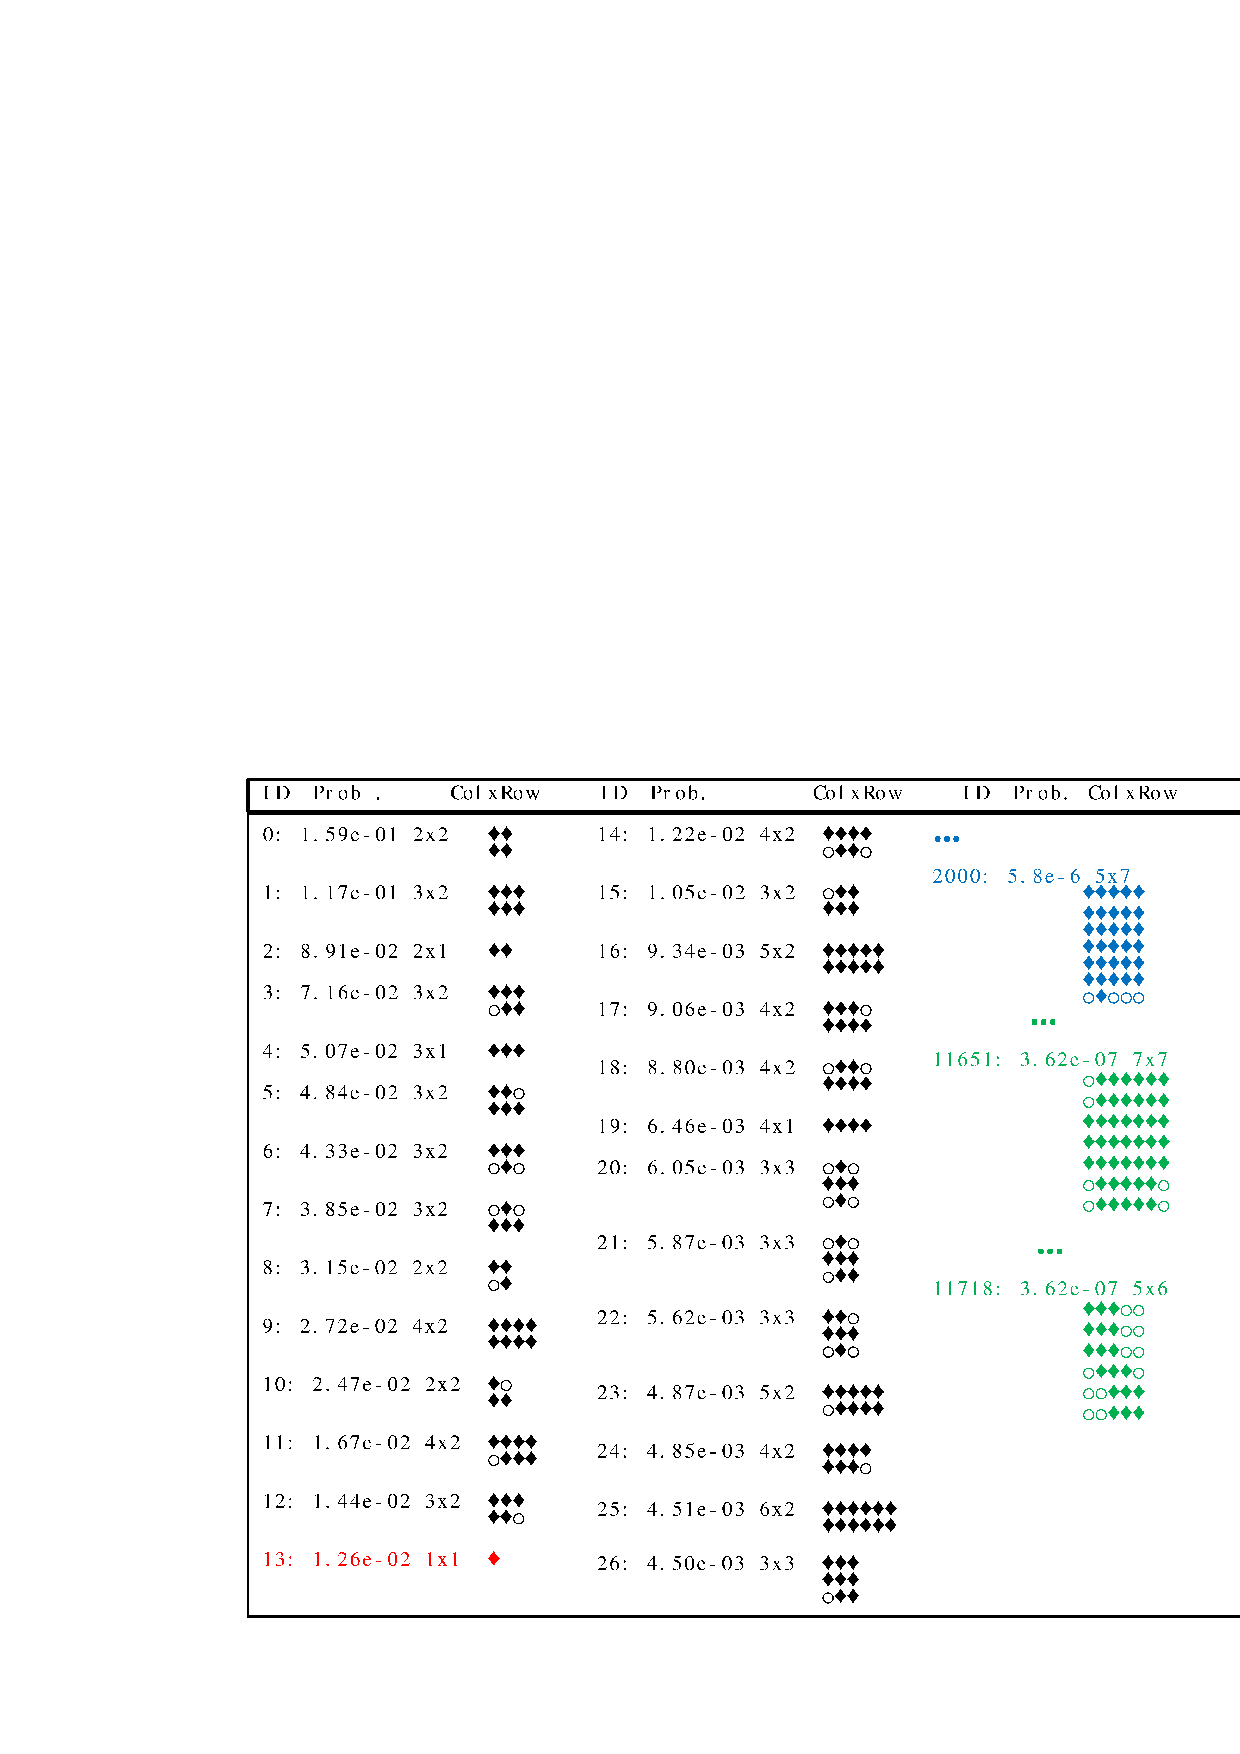
\includegraphics[trim=4.5cm 2cm 3.5cm 3cm , width=0.98\textwidth]{ITS/ClusPattDemo.pdf}
\caption{\label{fig:clpatt} 
Example of most and least frequent ITS clusters topologies. Column
"Prob" shows probability of given configuration while "Col$\times$Row"
is the dimension of smallest rectangle containing the pattern.}
\end{figure}

The probability
distribution of different patterns is shown on Fig.~\ref{fig:clpattHC}. We can assign dedicated ID to most probable
small cluster topologies and group a few patterns of rare large clusters with close topologies under the single ID.

\begin{figure}[h]
\centering
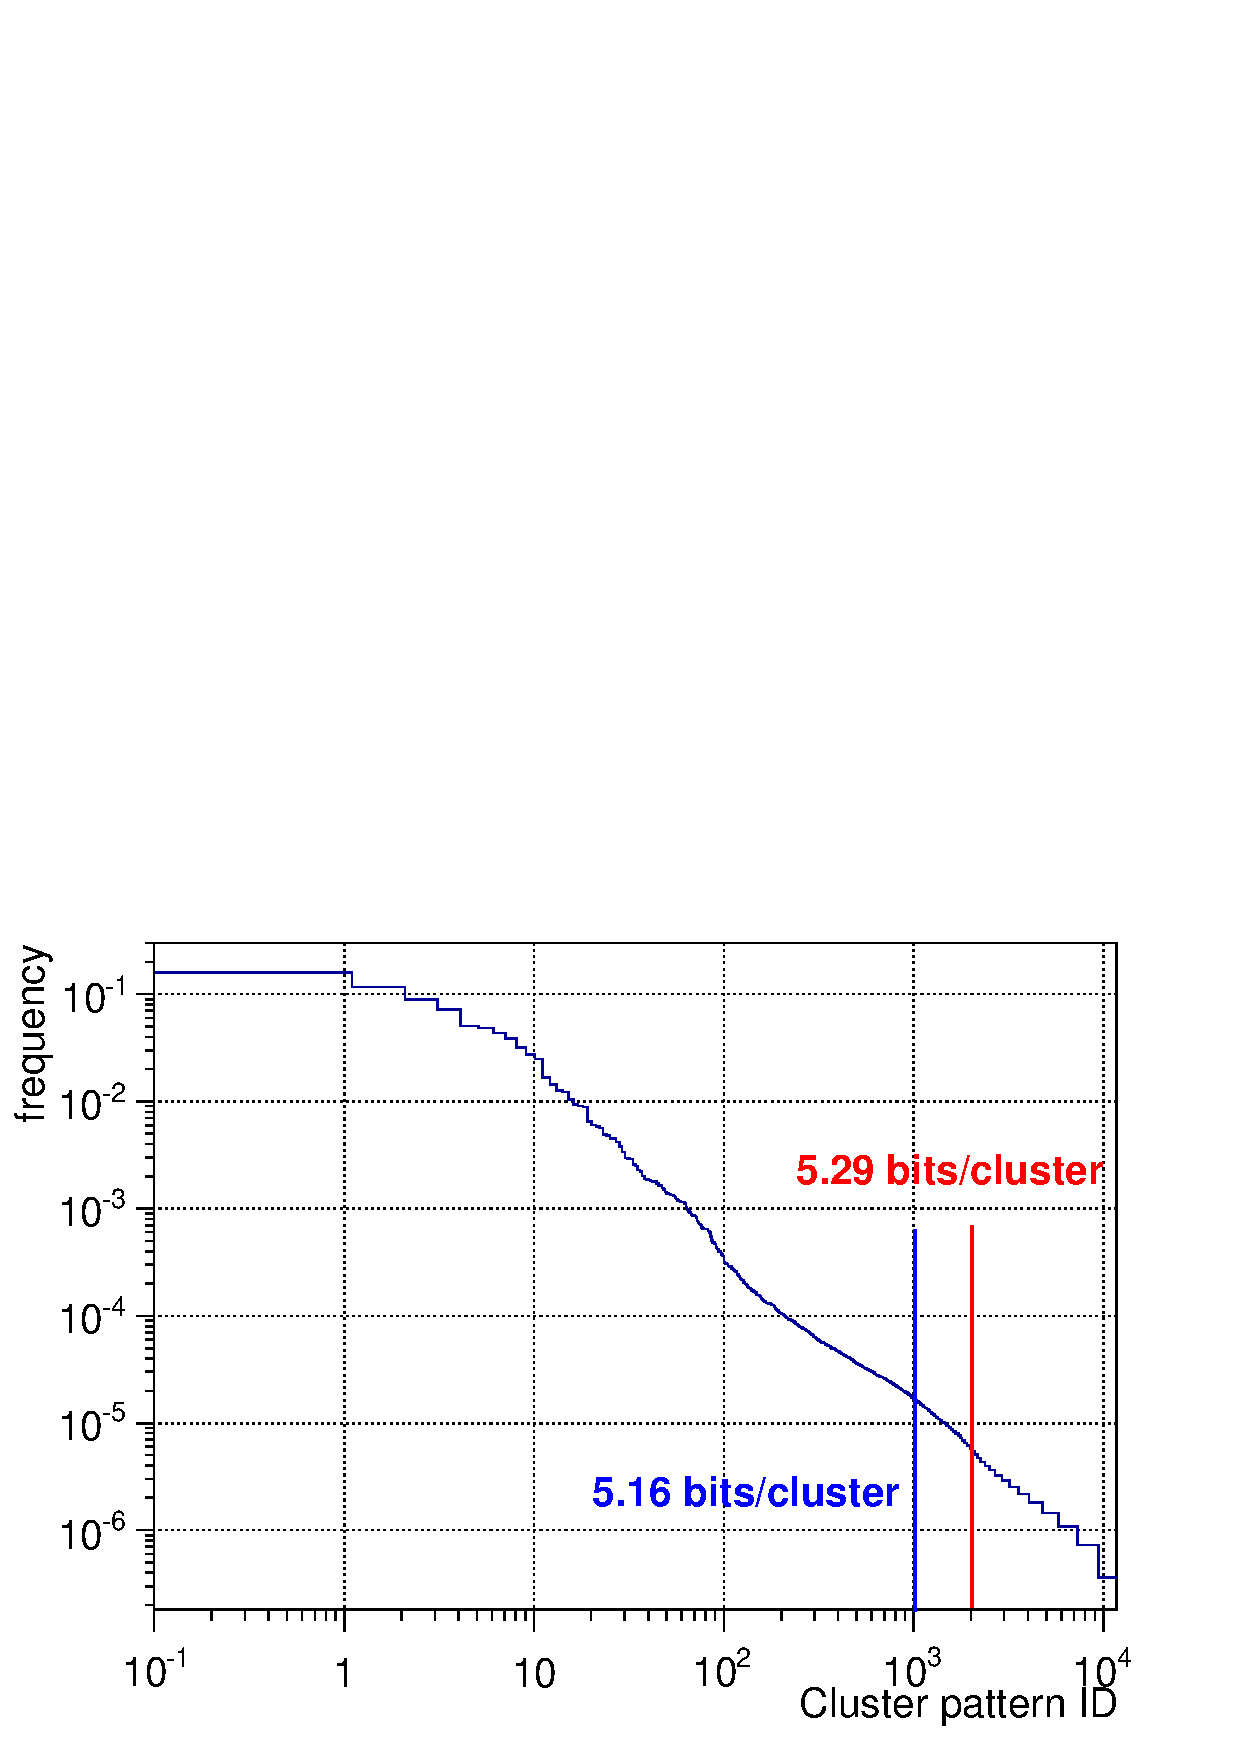
\includegraphics[width=0.9\textwidth]{ITS/ClusPattFreq.pdf}
\caption{\label{fig:clpattHC} 
Probability distribution of clusters with different ITS cluster topologies (see
Fig.~\ref{fig:clpatt}). The numbers refer to average (weighted) length
of the Huffman code for two choices of the number of pattern indices
to store.
Noisy pixels contribution is not accounted.
}
\end{figure}


If we define $\sim$2000 such IDs, using the Huffman coding we will need in average $\sim$5.3 bits per cluster if single-pixel
clusters are suppressed. In case we will need to keep the single-cluster pixels the average lenght of pattern ID record
will reduce to 1.8 bits for $10^{-5}$ noisy pixel probability.
Similarly, due to the ordering the probability distributions of $\Delta$\row and $\Delta modID$ are strongly non-uniform. 
Estimates show that we will need in average 1.2 bits per $\Delta modID$ and 7.3 bits per $\Delta$\row records in 
central \pbpb collision if single-pixel clusters are suppressed ($\Delta \row$ record will reduce to 
\TBD{<5 ?} if the single-pixel clusters are not suppressed). 
For peripheral collisions the compression factor for $\Delta \row$ deteriorates to \TBD{$\sim$10 and 7 bits
respectively}. The \col record will require $\sim$10.6 bits in average. 
Given that the $\Delta \row$ ($\Delta modId$) probability distributions strongly depend on the average number
of clusters in the module (readout frame) we will need to use different Huffman codes for the same type of record depending
on the multiplicity. 
In this way the storage clusters from single \pbpb collision will require $\sim$23 bits/cluster if the noise is rejected
and \TBD{$\sim$ 18} bits/cluster if the noise is kept. The corresponding preliminary estimate for the storage 
rate of \pbpb data at 50 kHz interaction rate is $\sim$5.3 GB/s discarding the single-pixel clusters while it would
stay $\sim$ 21 GB/s if the noise is not suppressed.

\subsection{ZDC calibration and reconstruction}
\label{ZDC:FLP}

For calibration purposes, the pedestal subtraction is no more needed since 
the baseline will be automatically subtracted from the signal. 
Concerning the energy calibration, similarly to what done in previous runs, 
the ZDC needs a significant sample of events using a trigger provided by the ZDC itself. 
The aim is to collect events coming from electromagnetic dissociation processes where the 
dominant emission channel results in the emission of single nucleons, allowing to perform 
the energy calibration and also to estimate aging effects on the detector. 
These runs will be standalone runs that should last few minutes and the needed frequency 
would be not less than every 2/3 days to monitor possible signal variation and resolution 
worsening due to aging.

The reconstruction will be similar to the current one, but simpler and faster since the code 
involving the pedestal subtraction will be avoided and the reconstruction algorithm will 
essentially consist in the energy calibration \TBD{in these standalone run and using the obtained
calibration coefficients for the energy estimates in the physics runs ???}

\subsection{PHOS calibration and reconstruction}
\label{PHOS:FLP}

%-----------------------------------------------------------------------------
\subsubsection{Reconstruction}

The ultimate goal of PHOS raw data reconstruction needed for further
physics analysis is producing reconstructed showers developed by
particles in the PHOS medium, with each cluster characterized by its
energy, coordinate, time and shower shape parameters. In general, PHOS
raw data reconstruction consists of two steps:
%
\begin{enumerate}
  \item Reconstruction of the amplitude and time of cells from the
    sampled digitized signal. It leads to a significant reduction of
    data volume, as from an array of up to 30 10-bit samples, only two
    floating-point parameters are derived, cell energy $E$ and time
    stamp $t$. In addition, a signal shape quality parameter can be
    derived from the fitting procedure which can be further used to
    assess the signal quality.
  \item Reconstruction of clusters of adjacent cells in PHOS. Each
    cluster, representing the shower developed by a particle
    interacting with the PHOS medium, is characretized by the
    reconstructed cluster energy, time with respect to the L0 trigger
    instance, cluster coordinate calculated from the cluster gravity
    center, and cluster shape parameters used later in analysis for
    photon identification.
\end{enumerate}
%
Further physics analysis operates with clusters which are used to
evaluate the 4-momenta of reconstructed photons and to calculate
identification probabilities to be a photon shower of clusters
produced by other type of particles.

Among possible implementation of on-line reconstruction procedures at
the FLP level, one can consider reconstruction of cell energy and time
from the sampled digitized data. It might be necessary to
significantly reduce the data payload produced by the PHOS detector to
the whole raw data stream. Estimated reduction of event size by this
signal shape reconstruction compared to full sampled raw data is a
factor of 10. This signal shape reconstruction can be potentially
implemented either at the FPGA of the PHOS front-end electronics, or
in HLT. Prototypes of HLT reconstruction are available in
\verb|aliroot| since Run-1.

Reconstruction of cluster from cells is not considered as an option
for physics analysis. Having cells in reconstructed data is necessary
for further offline calibration, also needed for tuning cluster fining
algorithms, for reconstruction efficiency calculation via embedding,
i.e. via merging simulated signals with real raw data. Cluster finding
cannot work in FLP, as cluster fining requires access to cells which
might be detected in different detector partitions.

%-----------------------------------------------------------------------------
\subsubsection{Calibration}

PHOS energy and timing calibration requires very large statistics
which cannot be accumulated in one physics run. Calibration is based
on physics observables such as $\pi^0$ peaks on invariant mass
spectra, average deposited energy in cells or time of cluster of
particles from the interaction point to PHOS. Although calibration
algorithms themselves are not feasible in on-line, filling and
accumulating histograms during data taking and storing them at an
external data storage might help in further offline calibration. 

\subsection{FIT calibration and reconstruction}
\label{FIT:FLP}

FIT calibration consist of 3 procedures:
\begin{itemize}
\item Slewing correction – required typically once per year; it is done either with the aid of the laser calibration 
system or/and with the physics data collected during the 1st day of data taking
\item Channel equalization – it is normally based on the first 20000 events; equalization can be done on FLP once a week
\item Global offsets – required to place T0A and T0C around zero. Calibration of these offsets is time-dependent 
and need information about full event. It can be performed on the FLP provided that the whole detector is processed
by the single FLP, otherwise, should be performed on the EPN.
\end{itemize}

The main purpose of reconstruction of the FIT data is to improve the precision of the
trigger parameters that are generated and available already online:
\begin{itemize}
\item Interaction time: calculated in FE as the average of the arrival time of the 1st signal generated on the 
A and C sides: (T0A+T0C)/2. Parameter equalization for trigger generation must be hardwired and therefore 
it’s accuracy is limited 
by the step size of the delay boxes and stability of the electronic units. 
During the reconstruction the delays can be equalized to higher precision and the interaction 
time can be extracted not just from the first signals but from the average arrival time on each side
(high precision interaction time is needed for particle identification using the TOF method).

\item The vertex position: defined as (T0A-T0C)/2. For trigger generation T0A and T0C are just the first 
signals on each side and instead of the numerical value only a binary value is given indicating the 
location of the interaction point either inside or outside of the predefined region. 
Reconstruction is needed to obtain the numerical value of the vertex position. 

\item The online multiplicity is only rudimentary and is accomplished with two pre-fixed comparator values 
indicating reaching the semi-central and central collision thresholds. 
During the reconstruction the sum of the amplitudes on each MCP sector can be extracted with a good 
precision giving not only the total value but also the pseudo rapidity distribution and the 
indication of the reaction plane. 
\end{itemize}

The reconstruction of the FIT takes negligible time and can be performed on the FLP (provided that both sides are
processed by the same FLP).


\subsection{TOF Data Reduction}
\label{sec:TOFDataReduction}
Even if the average payload per event of the TOF raw data format is quite limited it is not
completely optimized. This is due in particular to some intrinsic limitations of the existing hardware
of the TDC readout modules (TRM) which have on board legacy FPGAs (Actel ProAsicPlus\circledR APA750). 
With a much larger amount of data read-out a further optimization is obviously desirable.
However these cards will not be replaced as part of the upgrade program and an optimization with the current FPGAs
resulted impossibile.

The data format is currently made by a structure of control words (6 words for each TRM) encapsulating the hit
information (two words for each hit registered by the detector), providing addressing for hit encapsulated - if any - 
and validating the readout, including CRC controls on data potentially exposed to Single Event Upsets in internal staging FIFOs). 
This approach proved robust but due to the presence of these control words even an entirely ``empty'' event 
(no hit registered at TOF) has - however - a 21 KB raw data size. The control words contain also certain slow control information 
(such as temperatures of the cards and thresholds set on front-end cards) which can be stripped: the slow control part is already 
actually read-out via a devoted optical link and saved separately.

Several data reduction options are therefore possible inserting immediate processing at FLP level, with a greater
impact foreseen in \pp collisions, where the event multiplicity is smaller.
Different algorithms will be tested and their performance evaluated during RUN2 implementing them
inside the HLT. With respect to the standard numbers (e.g. maintaining the current format) 
we expect to achieve a 50\% data reduction in \pp and less in \pbpb (with data reduction performance
decreasing for the most central events where the pure 'hit payload' is however dominant). In Table~\ref{tab:InputRate} we tentatively
indicated a 20\% gain in \pbpb and we assumed an average 2000 hits multipicity at TOF in minimum bias. It must be taken into
account, finally, that the whole payload for TOF is also subject to some uncertainty in \pbpb depending on the actual bunch spacing scheme
that will be adopted by the LHC for heavy ions collisions.

\subsection{TOF Electronics Status}
\label{sec:TOFElectronicsStatus}
During PHYSICS runs, the TOF data will be checked to spot inconsistent data format, unexpected missing information, 
and errors flags raised by the electronics during the standard data decoding. This will allow to discard suspicious or not 
fully efficient parts of the detector's readout from data reconstruction. 

The information is going to signal which electronics channels were
actually enabled and properly functioning. Discarding the data from the malfunctioning channels will allow for 
further data reduction in addition to the one described in~\ref{sec:TOFDataReduction},
in charge of removing the header and control words of the parts of the detectors not containing any hit. 

The information will be stored as counters per channel locally on the FLPs while processing the data of one run. 
The run integrated information (channel efficiency) will be aggregated on all the FLPs and written on an OCDB-like 
storage at the end of the run to be used for Monte Carlo simulations. 
It will be an objects of $\sim 3$ kB per run.
%1 word (32 bits = 4 Byte) per TRM to track single TDCs; 38 TRM per SM; 18 SM --> 4 * 38 * 18 = 2.7 kByte 
% the info will be ON/OFF, using a threshold 

The processing time per event will be estimate using the already existing software implemented as DAQ DA and used 
during Run1.


\subsection{MUON}
\label{MUON:FLP}

%-----------------------------------------------------------------------------
\subsubsection{CRU}

Depending on the CRU FPGA available space and the availability of
competent (wo)manpower, we may think of reorganizing the MCH data in
ways that could help the pre-clustering stage performed in FLPs, or
even to do a pre-clustering on the CRU. As it's unclear whether all
this is doable at all, we will in this document assume nothing special
is done in the CRU.

\subsubsection{FLP}

On the FLP the very minimal set of operations that are foreseen
includes occupancy (MCH) and noisy channel (MID) maps computation.

Very likely, we should also be able to perform pre-clustering on the
FLPs. The pre-clustering is a simple clustering algorithm which groups
adjacent pads, irrespective of their charges, into preclusters. The
current (recursive) implementation used in AliRoot 5 accounts for
roughly 20\% of the total clustering time. Very initial investigations
about possible optimizations of the way we access/store pad
information (e.g. using more static data structures with respect to
the current ones) have shown that we can most certainly gain a factor
20 in speed for the pre-clustering stage, getting to about 2 ms per MB
\pbpb event on one core of an Intel i7 @ 2.3 GHz processor (excluding
I/O). Further speedup would require moving part of the pre-clustering
into accelerator cards, e.g. FPGAs (hosted by the CRU or the FLPs
themselves, whatever the case may be). Manpower to investigate this
option is being searched for.

Whether or not the next processing stage, namely the clustering, can
fit within the FLPs, is an opened question. We first have to assume
that the MCH FLPs will see complete detection elements (either slats
or quadrants), otherwise we don't have the relevant information for
clustering. Then, if we assume also that they'll be equipped with GPUs
(or other "accelerator" like Xeon Phi) then the plan is to convert the
clustering stage to a GPU version, where we can only guess to be able
to gain a factor 50 in speed. Admittedly, without even an early
prototype of that version, the speedup factor is more a wish than a
real estimate... But even without a GPU version we expect to be able
to improve the current CPU implementation, e.g. using the same static
data structures as in the pre-clustering. Whether or not such an
implementation would fit in a FLP remains to be demonstrated.

For MID, it is still unclear whether or not anything will have to be
developed at the FLP level. In the case we are able to reconstruct at
the EPN level all the MCH tracks (see next section) then nothing is
really needed for MID at FLP level. On the contrary, if we need an a
priori selection of the events to be fully reconstructed by MCH (in
the case the full reconstruction is found to be too slow to cope with
50 kHz event rate), then we will need to get the computation of a
trigger-like decision somewhere in the chain. We know we will get
exactly one FLP for MID, so that FLP will see all the MID data at
once, and hence can compute a trigger-like decision. Given the current
uncertainty of the achievable speed of the full MCH reconstruction, we
do plan to investigate, during Run2 already (within the HLT farm), an
implementation of the trigger decision, that could be used to select
which events should be fully reconstructed.

The data reduction that can be achieved at FLP level is currently
largely unknown. Lossless compression (using e.g. Huffman coding) of
the pad data has not been investigated yet. In the worst case, we will
in fact slightly increase (by $\sim$ 3\%) the data volume (after pad cleaning), as we'll be
adding some data to mark the pre-clusters : we would for instance
re-order the digits by pre-cluster and thus need some boundary words (assuming 16 bits would be enough)
to separate the digits from different pre-clusters. This may tell us that the clustering
should not be done at the FLP level, even if fast enough, but on EPNs.

\subsection{HMPID calibration and reconstruction}
\label{HMPID:FLP}

The ALICE-HMPID is devoted to the identification of charged hadrons. It consists of seven identical RICH counters,
with liquid C$_{6}$F$_{14}$ as Cherenkov radiator (n = 1.299 for $\lambda_{ph}$ = 175 nm). Photons and charged particles detection is performed by a MWPC, coupled with a pads 
segmented CsI coated photo-cathode. HMPID provides 3 sigmas separation for pions and kaons up to $p_T$ = 3 GeV/c and for protons up to $p_T$ = 5 GeV/c. PID is performed 
by means of photon emission angle measurement. Photon emission angle reconstruction can be divided in two steps. In the first step from raw data the coordinates and 
the charge values of the fired pads have to be retrieved, from these informations the clusterization algorithm can create clusters. 
The second step requires the tracks to be extrapolated from the central tracking devices of ALICE (ITS, TPC) and associated with the corresponding cluster of the minimum
ionizing particle in the HMPID cathode plane. Starting from the cluster centroid one has to reconstruct the angle under which the photon causing it could have been emitted if belonging to the given track.

It can been foreseen that for the online-reconstruction procedure, HMPID clusterization can be executed at FLP level. No calibration is needed at this step, the pedestal subtraction will be executed directly by the RO electronics. The pedestal values will be calculated 
in the CALIBRATION runs using using dedicated script with a procedure quite similar to that already used in RUN1. 
 

%-------------------------------------------------------
\section{Calibration, reconstruction and data reduction on EPN's}
\TBD{This section describes for each detector 
\begin{itemize}
\item Feasibility of final online reconstruction 
\item What is done on the EPN's, description of algorithms (if any)
\item Estimates on the processing rate
\item Estimates on the data rate to permanent storage
\end{itemize}
}

\subsection{ITS}
\label{recoEPN:ITS}

In opposite to Run1 situation, where most of the tracks in the ITS are found as prolongation
of TPC tracks, in Run3 the TPC itself needs ITS tracks in order to perform final calibration of
the space charge distortions. Therefore, a standalone tracking in the ITS needs to be performed.
The principal requirement to the code used for ITS tracking is the speed, since at least the part
of reconstuction should be performed in real time.
The algorithm that is currently under study is based on a Cellular Automaton (CA) (see 
Alice ITS TDR \cite{refITSTDR} and \cite{refCA1, refCA2}). Since at the moment no working code exists 
for the ALICE ITS, for the estimates of its performance we have to rely on the benchmarking done by the
CBM collaboration for their Silicon tracker made of 8 planes of microstrips. 
The reconstruction consisted of three passes by the algorithm, the first two corresponding to a search of 
high and low \pt tracks converging to vertex region and the third one for the secondary tracks (w/o requirement
of the convergence to the vertex).
The estimated reconstruction efficiency is shown on Fig.~\ref{fig:ITSreceffCBM} (left) 
for single central Au-Au collision as function of the track momentum and (right) as function of the multiplicity
(created by piling up the space points from many minumum bias collisions). 

\begin{figure}[h]
\centering
\includegraphics[width=0.48\textwidth]{ITS/IK_CBMeff.pdf}
\includegraphics[width=0.48\textwidth]{ITS/IK_CBMeffmult.pdf}
\caption{\label{fig:ITSreceffCBM} 
Reconstruction efficiency of CBM CA tracker for single central Au-Au event (left)
and as a function of multiplicity obtained by piling up multiple collisions (right).
}
\end{figure}

Fig.~\ref{fig:ITSrecotimeCBM} shows the reconstruction time as a function of the multiplicity 
in the detector acceptance, performed on the single core of the Intel E7-4860 at 2.27 GHz processor. 
The multiplicities expected in the Alice ITS
for central \pbpb collision and in the single ITS readout cycle of 30\ums at 50 kHz interaction rate are shown
by the red bars. The timing of $\sim$0.2 s for reconstruction of average readout cycle seen on this figure cannot
be directly applied to Alice case. First of all, CBM, being a fixed target experiment, sees in average tracks of 
higher momentum that Alice. While Alice needs to perform the tracking up to momenta (e.g. \pt) below 100~MeV/c,
the CBM reconstructed momentum spectrum stops at momentum $\sim$250 MeV/c. Given that the reconstruction of the 
low momentum tracks is most time consuming, one should expect faste reconstruction in the CBM
tracker than in the Alice ITS. As a tentative estimate we assume that the average ITS readoud cycle (with multiplicity
equivalent to that of 1.5 minimum bias \pbpb collisions at 50 kHz interaction rate) can be reconstructed in less than
1 s on a single core. 

\begin{figure}[h]
\centering
\includegraphics[width=0.80\textwidth]{ITS/IK_CBMrecotime.pdf}
\caption{\label{fig:ITSrecotimeCBM} 
Results of benchmarking for reconstruction time versus number of 
tracks in the acceptance for CBM CA tracker (on a single core of the Intel
E7-4860 at 2.27 GHz processor).
}
\end{figure}


As it was mentioned 
in Sect.~\ref{ITS:datarate}, one cannot exclude that the cluster data will be dominated by the random noise in
the pixel detectors, in which case even after the compression described in Sect.\ref{recoEPN:ITS} the rate
of the ITS cluster data will exceed 20 GB/s, factor 2 higher than the maximum target rate for storage.
Therefore, the aim of the on-line reconstrcution is not only finding the tracks in the ITS and providing a 
constraint for TPC calibration
but also the reduction of the cluster data to the level acceptable for the permanent storage. 
Approximately 50\% of clusters produced by the primary and secondary particles are not used by the 
reconstructed tracks, hence can be rejected before the storage (provided that the reconstruction reaches its
maximum efficiency). This fraction will increase even further if the cluster data are dominated by the noise,
guaranteeng the reduction of the storable data rate to acceptable level. 

In case the full reconstruction of the ITS will appear to be too slow for the real-time processing, it should be
performed either in quasi-online (i.e. data is bufferized locally on the EPN and reconstructed by the
beginning of the next fill) or the offline mode. For this scenario we are considering an alternative way of 
the cluster reduction which does not require full real-time tracking. The idea is to keep only those clusters
of the outer 5 layers (containing 95\% of noise clusters)
which can be bound to helical triplets pointing to the proximity of the interaction region. Since binding the
clusters in such triplets is a necessary step also in the CA tracker, one can consider such a data reduction
in the incomplete reconstruction as a rescue mode of the full tracking. The preliminary estimates of data
reduction by combining clusters to triplets is XXX\% and YYY\% for the scenario with $10^{-5}$ noise and 
without the noise respectively.

\subsection{TPC reconstruction, calibration, and data compression}
\label{sec:calibreco:reco:overview}

The ALICE upgrade requires a major change of the computing concept in
order to be able to process and store the large amount of data
produced in \pbpb collisions. The main contributor to the data volume
will be the TPC operated in continuous readout mode.
Most of the data processing and reconstruction will be performed on the
computing cluster of the new online systems~\cite{ALICELOI}.
New requirements to calibration and reconstruction algorithms emerge in
terms of running stability, processing time, memory consumption, as well
as parallelizability on different levels.
A massive use of hardware co-processors, such as FPGAs for the early
processing steps, as well GPGPUs\footnote{General-Purpose Graphics
Processing Units (GPGPUs)} for the later processing is foreseen.
These requirements build strict constraints on the data reconstruction
and calibration, as well as data compression.


%===================================================================
% \subsubsection{The TPC in the general reconstruction scheme}
\subsubsection{Overview of the TPC reconstruction scheme}
\label{sec:calibreco:intro:reco}


The choice of the reconstruction algorithms is strongly driven
by the constrains of the online processing.
However, in the discussion below we will focus on demonstrating the
overall strategy and the general feasibility of online reconstruction
under the operational conditions expected in \run{3}.

A two-stage process, as depicted in
\figref{fig:calibreco:calib:intro:flow}, is foreseen for the online data
processing.
The first stage (see \cite{TPCTDR}) will focus on
cluster finding and the association of clusters to tracks, which are
needed in order to perform the necessary data size reduction.
% This stage must be performed online.
The compressed data will be written to permanent storage.
The reconstructed tracks have sufficient precision to allow the matching
to the external detectors, mainly ITS and TRD, to improve the quality of
the calibration during the next reconstruction stage.

\begin{figure}[htp]
  \begin{center}
    \includegraphics[width=0.9\textwidth]{TPC/CalibSteps}
    \caption[Schematic outline of the calibration flow]{Schematic
      outline of the calibration flow during the data-taking and
      reconstruction process.}
    \label{fig:calibreco:calib:intro:flow}
  \end{center}
\end{figure}

The second reconstruction stage will also be performed on the online
computing cluster, but in an asynchronous mode and can thus be repeated
at any time.
It aims at a further improvement of the data quality, in particular in
terms of the space-charge distortion calibrations, and employs
information from external detectors as well as more detailed calibration
data.

\subsubsection{Data size and data compression}
\label{sec:calibreco:intro:compression}

After zero suppression on the level of the \fee, the average TPC raw
data size in \minbias \pbpb interactions is $\sim20\,$MB.
At an interaction rate of
50\,kHz, this would result in an input rate of about
1\,TB/s to the online systems, and a total amount
of
3\,EB ($10^{18}$\,Byte) of TPC data in \run{3}. Such numbers
exceed the predicted available bandwidth and storage space by a large
factor. Thus, in order to permit permanent data storage, additional
compression on top of zero suppression to below 1\,MB per
interaction is required. This can be achieved by two levels of pattern
recognition that are performed in the online systems.

The zero-suppressed raw data are decoded at the input to the online
farm, where the raw data digits (arrival time at the \fee and signal
amplitude) are associated with the corresponding geometrical position
(pad row and pad coordinates). Cluster finding is performed
on the digits, which produces three-dimensional charge clusters.
This first step is carried out on the FLPs.

As the radial coordinate is fixed by the well-separated pad
rows, cluster finding is reduced to a two-dimensional problem in the
pad--time plane.
A two-dimensional algorithm, as used in the current TPC offline cluster
finder, scans the pad--time plane for charge maxima using a
sliding window. It allows a good (charge) separation of close-by
clusters. A different method is based on a one-dimensional algorithm,
as used in the current HLT system. It processes the pads sequentially,
which allows to find the maxima within neighboring pads on the same
pad row. In this case the separation of close-by clusters is done
separately in both dimensions. The algorithm allows massive
parallelization and, therefore, an easy implementation into an
FPGA\footnote{Field Programmable Gate Array (FPGA)}. It is the
baseline solution for \run{3}, as it fits the necessity of an early
data reduction already at the input to the online systems.

The cluster finding is accompanied by a further compression step based
on intelligent Huffmann Coding~\cite{4051119Huffmann}  of selected
parameters.

Such a compression scheme has already been applied to TPC data during
the 2011 \pbpb data taking in \run{1}, resulting in a data compression
factor of $\sim4$ as compared to zero-suppressed raw data. Further
optimizations of the
cluster data format and of the compression algorithm for \run{3} will
allow a total data reduction by a factor five to seven during the
cluster finding step~\cite{ALICELOI}.

A further reduction in data size can be performed on the EPNs with a
tracking step, where clusters are assigned to tracks.
This step, allows to remove clusters that are not associated to
physics tracks (e.g.~clusters from delta electrons and noise clusters)
from the data stream. The possible reduction factor, based on the
experience from the past data taking in \run{1}, is of the order of
two. The tracking step also enables more advanced transformation
schemes to optimize the parameter distributions for entropy encoding,
as well as the possible replacement of some of the individual cluster
parameters by track-based properties. We estimate the further
reduction potential to be on the order of two to three.

In total, the envisaged compression factor in the online system is of
the order of 20, resulting in an average data size per interaction of
<1\,MB. This will lead to a storage rate of
$\sim$50\,GB/s and a total amount of
$\sim$150\,PB
of stored data during \run{3}.
To store the cluster information associated to the reconstructed tracks
is an advantage, allowing a possible re-calibration of individual
clusters at a later stage and, therefore, an improvement of the TPC
performance.
A summary of the consecutive data compression factors is presented in
\tabref{tab:reco:compression}.

\begin{table}[hbt]\footnotesize
  \centering
  \begin{tabular}{l  c  c}
    \toprule
    Data Format                     & Data Compression Factor & Event
Size (MByte) \\
    \midrule
    % Raw data                               &  1    & 700   \\
    % Zero Suppression (FEE)                 &  7    & 100   \\
    % Associate digits to                    &  5    &  20   \\
    % relevant interaction (Logical)         &       &       \\
    Zero Suppression (FEE)                 &       & 20   \\
    Clusterization (FLP)                   & 5-7   &  3    \\
    Remove clusters not associated         & 2     &  1.5  \\
    to relevant tracks (EPN)               &       &       \\
    Data format optimization               & 2-3   & $<$\,1 \\
    \bottomrule
  \end{tabular}
  \caption[Event size and data compression factors]{The TPC event size
    and data compression factors for the different data compression
    steps performed in the front-end electronics and the online
    systems. Table adopted from \cite{ALICELOI}.}
  \label{tab:reco:compression}
\end{table}


\subsubsection{Calibration requirements}
The most important calibrations for the track reconstruction are the
correction of the cluster distortions induced by space charge and the
drift velocity.
The two reconstruction stages described above have different
requirements on the precision of the calibration data.

\paragraph{First reconstruction stage}
For the first stage, which focuses on data compression, the calibration
quality has to be good enough to perform a cluster to track association.
This translates into a precision for the cluster corrections due to
distortions induced by space charge to the level of the intrinsic
cluster resolution ($\mathcal{O}$(1\,mm)).
This can be reached by using a long term average map of the space
charge distortions, which follows changes in the operating conditions
like the instant luminosity and the detector configuration.
Such a map can be obtained from a high statics, high \pt sample of
external detectors and is expected to be updated on the level of tens
of minutes.
The average map will need to be scaled to the instant average ion
density in the TPC, which is driven by the number of collisions and the
collision centrality during one full ion drift (160\,ms).

For the drift velocity a precision of $\mathcal{O}(10^{-4})$ is
required.
To obtain this requirement, a scaling with the current temperature and
pressure inside the TPC is sufficient.
Additionally the gain variations of the readout chambers due the change
of the gas density will be corrected.


\paragraph{Second reconstruction stage}
The second reconstruction stage will provide the full tracking
resolution for physics analyses and requires a space charge correction
to the level of the intrinsic track resolution of
200\,\textmu m.
In order to reach this level of precision, space charge correction maps
will need to be calculated with high granularity in space and time.
The update interval for these maps is estimated to be on the level of a
few \textmu s ($\mathcal{O}(2-5)$) and driven by the
fluctuations of the space charge \cite{TPCTDR}.

To follow the fluctuations it is foreseen to have information of the
readout currents of the TPC of the last 160\,ms integrated in
steps of 1\,ms available during the reconstruction.
For the readout currents, the analog currents measured at the high
voltage (HV) sectors of the GEM system as well as the digital currents
in form of the ADC counts will be necessary.
The granularity of the HV sectors is about 100 per readout sector, for
the digital currents information from each individual channel (total
$\sim$553\,k).

Additionally, the interpolation of track segments from the ITS and TRD
will be used to calibrate residual distortions.
The drift velocity will be treated as an additional parameter in the
fitting procedure and allow to reach the required final precision of
$\mathcal{O}(10^{-5})$.

Another complication is given by the expected stability of the gain of
the readout chambers.
The current assumption is that in order to obtain the required energy
loss resolution for particle identification gain calibration will need
to be performed on the sub-minute level.

\paragraph{Summary}
In summary the following requirements are set for the availability of
information during the data reconstruction.
\begin{itemize}
  \item Well aligned ITS and TRD detectors
  \item Standalone tracking of ITS and TRD
  \item TPC temperature and pressure values online
  \item Integrated TPC currents in the data flow
  \begin{itemize}
    \item Integration interval: 1\,ms
    \item Data history: last 160\,ms
    \item Granularity for digital currents: per pad
    \item Granularity for analogue currents: per GEM HV channel
  \end{itemize}

\end{itemize}


% \begin{table}
%   \centering
%   \begin{tabular}{c c c}
%     \toprule
%     calibration type  &  & \\
%     \midrule
%     drift velocity    &  & \\
%     space charge      &  & \\
%     \bottomrule
%   \end{tabular}
%   \caption{bla}
%   \label{tab:TPC:calib:requirements}
% \end{table}



\subsection{TOF Detector Status}
\label{sec:TOFDetectorStatus}
At the level of EPNs, TOF collects the information coming from previous calibration runs (NOISE, running before
PHYSICS, the information of which is expected to be available to all EPNs in some way during the subsequent
PHYSICS runs), detector configuration (high/low voltage status, electronics and trigger configuration) from the
equivalent of the Run1 Detector Control System. The aim is to further reduce the data size discarding 
unwanted hits coming from the channels that were either OFF (no LV and/or HV) or flagged as noisy. 

This information (noise and detector configuration) will have to be exported once per run somehow to the 
OCDB-equivalent structure to be available for Monte Carlo simulation. A Run1 preprocessor-like process will be needed to 
prepare the object from DCS and NOISE runs (i.e. not necessarily running on EPNs during data taking). The 
estimated size per run is $~160$ kB.
%1 byte per channel

The estimated CPU time for the process is to be tested in the same framework as the data reduction described
in~\ref{sec:TOFDataReduction}.
\subsection{TOF Time Calibration}
\label{sec:TOFTimeCalibration}
The collection of the information needed to perform TOF time calibration 
can start only at the stage when the TPC tracking performance is sufficiently stable and accurate to allow
reliable extrapolation to TOF and matching with TOF signals. The TOF time calibration includes the measurement
of a few time offsets with different granularity, of which single channel offsets and channel time slewing parameters are 
the most demanding in terms of statistics. These parameters are expected to be constant in time, being related only
to the hardware configuration, and can be obtained in the foreseen commissioning phase at the beginning of Run3. 
On the other hand, it cannot be excluded that hardware interventions may happen, requiring, as a consequence, 
an update of such parameters. For this reason, different approaches are being investigated in order to keep 
track of the calibration information which might be needed for update and adjustment. One possibility could be 
to store on a run by run basis histograms or trees, with a preselection on the tracks. 

The same calibration information will in addition be used in order to monitor the behaviour of the detector
by looking at the distribution of the time signals per channel. Channels whose signal is unstable or 
badly behaving should not be used for physics analysis . For instance, this could be due to an unexpected 
loss of configuration of the electronics or to data corruption not tracked down during the previous calibration 
steps~\ref{sec:TOFElectronicsStatus}.
%Still under investigation which algorithm could be implemented so that this is done automatically. 

The possibility to use the time calibration only at analysis level is being evaluated. This would imply that in case TOF
signals from adjacent channels (generated by the same traversing particle) have to be merged in a single
cluster, this can only happen at analysis. 


\subsection{MUON}
\label{MUON:EPN}

%-----------------------------------------------------------------------------
At the EPN level, we will perform the clustering (if not done at FLP
level), the tracking (of both MCH and MID), the MID-MCH matching and,
optionally, the computation of preliminary steps for the alignment
(typically computation of derivatives).

The biggest time consuming part of the current MCH tracking is the
access to the magnetic field values during extrapolations. We plan to
attack the problem by a) decreasing the number of times we access the
magnetic field values and b) decreasing the time spent during each
access. No speedup estimate is currently available though. The MID-MCH
matching should be of little influence as far as computing time is
concerned.

The strategy to reduce the EPN output data volume is multifold.

First, if we assume we have/need a MID trigger-like decision (done in
FLP), then we can reject roughly half the events (those which do not
have any MID tracklet). This corresponds to the situation of Run1 with
the AllPt (0.5 GeV/c) MTR \pt threshold.

Then we can increase the rejection factor by increasing the \pt
threshold (e.g. in Run1 we used a threshold of 1 GeV/c for \pbpb, in
which case we reduce by 6 the number of events to be written), at the
expense of the physics cases we'll be able to cover if we increase the
threshold too much.

Lastly, there's a very agressive option in which we trust the
clustering enough to drop completely the original pad information and
keep only the cluster data (identifier, local position, resolution in
x and y, which would amount to about 160 bits per cluster). This is of
course a very dangerous option as there's no way back (still we could
redo the tracking offline)... Assuming a mean number of pads (~3000
from Run1 data\footnote{3000 pads after removing the bad pads, so that the good pad information alone is below the 1.5 GB/s of the raw data...}) 
and a mean number of clusters per MB event (~400,
again from Run1 data), we'd achieve a further reduction of a factor 3
(3000 pads x 64 bits versus 400 clusters x 160 bits) of the cluster
data.

The track data size should be small, as we expect few tracks per event : $\sim$ 2 tracks/MB event in Run1 \pbpb leading to 9 MB/s assuming 1500 bits for one track data including references to clusters.

Table \ref{tab:data reduction values} summarizes the reduction factors using different strategies. Notice however that some reduction strategies come at a price, which we don't  necessarily know yet. For instance, let's take the "Keeping complete tracks and all clusters" strategy as the baseline, which seems to offer a very reasonable trade-off between flexibility (we can still redo the tracking at a later stage if need be) and data reduction. If the pad information is dropped, then we trivially know that clustering cannot be redone, but we still have to investigate how to deal with embedding at the cluster level, which is an important tool to assess multiplicity effects on efficiencies. For instance, could we go back, in some way, from a cluster to its pads (using the Mathieson charge distribution, under the assumption that the clustering is somehow "reversible" - to be carefully validated, of course-) ? Or should we simply plan to store the full information, including pads, for a fraction of events ? Or should we plan to embed the embedding into the online reconstruction itself ? After all, the simulation and reconstruction of one single MC particle, being a single muon or a resonance, might not increase the CPU budget by a big factor, depending on the progress on the simulation front (CWG8). But that would mean loosing a lot of flexibility : we would for instance need to decide a priori which particles (\jpsi, $\upsilon$, etc...) to embed, so the implications need to be carefully investigated...

On the other hand, depending on the exact storage bandwidth budget allocated to the Muon Spectrometer, we might be able to retain all the information (pads, clusters and tracks) by choosing an adequate event rejection (e.g. accepting only 1/6th of the events, achieved with a 1 GeV/c $p_{\rm{T}}$ threshold, would lead to 700 MB/s to storage).

\begin{table}
\centering
\begin{tabular}{|p{4cm}|p{3cm}|p{3cm}|p{3cm}|p{3cm}|}
\hline
Data reduction method & output of FLPs (MB/s) & output of EPNs (MB/s) w/o event rejection & total reduction factor (w/ event rejection) \\
\hline
\hline
None & 1200 &  2100 & 1.14 - 3.4  \\
\hline
Keeping complete tracks and their associated clusters only & 1200 & 26 & 90 - 270 \\
\hline
Keeping complete tracks and all clusters &  1200 & 400 & 6 -  18 \\
\hline
\end{tabular}
\caption{\label{tab:data reduction values}Summary of data reduction strategies. The raw data rate (input to FLPs) is assumed to be 1500 MB/s for 50 kHz MB. The event rejection factors are assumed to range from 2 to 6, depending on the $p_{\rm{T}}$ threshold chosen.}
\end{table}

\subsection{HMPID calibration and reconstruction}
\label{HMPID:EPN}

At the level of EPNs the final step of the angle reconstruction has to be executed. The final fully calibrated tracks from TPC are needed at this step for the HMPID reconstruction.
From the DCS have to be retrieved the following parameters: the HV sector voltage values, the chamber pressure values, the radiator temperature values and transparency. 
This information have to be also exported once per run somehow to the OCDB-equivalent structure to be
available for Monte Carlo simulation. A Run1 preprocessor-like process will be needed to prepare the object from DCS. 
 

\subsection{EMCal Reconstruction}

The energy deposited by the particles in the towers produces scintillating light that is propagated with optic fibers through the different layers to APD placed at the base of the cells. The APDs amplify the signal and generate an electronic pulse shape that is stored in the raw data format which consists of a series of so-called time samples with 10-bit ADC counts per channel. Each time bin is 100 ns wide, corresponding to a 10 MHz readout.
The signal has a Gamma-2 shape. From this pulse shape, we extract the signal amplitude and the arrival time. The pulse shape is fitted (\bf{fitter to be chosen and described here? right now, Run1-2 TMinuit fitter, for Run3 use  HLT fast fitter  AliCaloRawAnalyzerPeakFinder?}), and those 2 values are extracted and form what is called as digits.

A particle produces signals in different towers (electromagnetic shower expands more than its Moli\`ere radius which is a cell size). The next step is the formation of clusters of cells that belong to the same particle, although depending on the energy, granularity, clusterization algorithm or event type, those clusters might have contributions from different particles. The default algorithm in pp collisions is a simple aggregation of neighboring cells until there is no more cells above a certain energy threshold (named {\it clusterizer V1}). In case of Pb-Pb collisions environment, where particle showers merge quite often, we apply another algorithm that aggregates cells to the clusters until reaching a cell with more energy than the precedent (named {\it clusterizer V2}). Depending on the analysis type, one might want to use one or the other clusterization type. For this reason, a re-clusterization is also possible at the analysis level using as input the tower information stored in the analyzable data.

Once the cluster is defined, we calculate cluster parameters, shower shape parameters, that will help at the analysis level to identify each cluster as one particle type. Also, we compare the cluster position information with the propagation of tracks measured in the central barrel to the EMCAL surface, to identify the clusters generated by charged particles.

The final analysis objects, ESDs and AODs, contain all the cluster and cell basic informations allowing to redo the clusterization if needed at the analysis level.

The most expensive steps in the EMCal reconstruction are the pulse shape fitting  (this might not be the case when using fast fitters like HLT one) and the cluster-track matching (\bf{fshould we give numbers? this depends a lot on the pp, PbPb})


\subsection{EMCal Calibration}

\subsubsection{EMCal $\pi^{0}$ calibration}
The energy calibration relies during data taking on the measurement of the $\pi^{0}$ mass position per cell. Each tower has a calibration coefficient. In what follows, a calibration parameter is equal to the result of the fitted mass over the PDG mass value, where the fitted mass denotes the mass given by a gaussian fit on the $\pi^{0}$ invariant mass peak distribution in a given tower (plus a combinatorial background, fitted by a 2nd degree polynomial).
About 100-200 M events EMCAL (L0) triggered (trigger threshold at 1.5-2 GeV) allow to calibrate a majority of the towers ({\bf the statistic might change with the increase of colliding energy but of the same order}). The towers located at the borders of the super-modules and those  behind the support frame (about 5 columns per SM) have much fewer statistics and would need a minimum of 150 Mevts (probably more). It is to be noted that the run-to-run temperature variations change the towers' response in a non-uniform way, i.e. the width of the $\pi^{0}$ peak increases, and the mean $\pi^{0}$ mass is shifted differently for the various towers. Also the $\pi^{0}$ mass shifts to lower values for the towers with material in front, due to photo-conversion close to the EMCAL surface.

A few iterations on the data, 3 to 5, obtaining in each iteration improved calibration coefficients, are needed to achieve a good accuracy (1-2\%). Since the online calibration has a strong effect on the trigger efficiency, the voltage gains of the APDs are varied after each running period, to get a uniform trigger performance. 

This calibration, since it needs a large amount of statistic, will run after the data is reconstructed and it will run like an analysis task. The calibration factors obtained will be applied at the analysis level.

\paragraph*{$\pi^{0}$ Calibration Procedure\\}

Since $\pi^{0}$s decay into 2 gammas, their invariant mass is calculated from the energy of 2 clusters (and angle between the clusters). The position of the invariant mass peak of a tower therefore doesn't depend only on its response and calibration coefficient, but also on an average of the responses and calibration coefficients of all the other towers of the SM, weighted by  how often they appear in combination with a cluster in the considered tower. The 2nd effect, of weaker magnitude maybe, originates from the fact that a cluster most often covers more than the considered tower. To simplify the calibration process, the calibration coefficient is calculated as if the whole energy of the cluster was contained in the tower of the cluster which has the largest signal. So the position of the invariant mass peak of a tower also depends on an average of the responses and calib coeffs of its neighbouring towers. For these reasons, the calibration of the calorimeter with the  $\pi^{0}$ is an iterative procedure :
\begin{itemize}
\item Run the analysis code on this data to produce the analysis histograms per tower and a 1st version of the calib coeffs.
\item Look at the fits on the towers invariant mass histograms and discard the value (or set it by hand) of the calib coeff of the towers for which the fit can't be trusted.
\item Create a 1st set of OCDB coeffs.
\item Reconstruct the $\pi^{0}$'s with these OCDB coeffs.
\item Run the analysis code on this data to produce the analysis histograms and a 2nd version of the calib coeffs.
\item Look at the fits on the towers invariant mass histograms and discard the value (or set it by hand) of the calib coeff of the towers for which the fit can't be trusted.
\item Create a 2nd set of OCDB coeffs.
\item Etc..., until the invariant mass is satisfactory in all the towers, i.e., the calibration factor does not change in the next iteration more and 1\%.
\end{itemize}
When the statistics is enough, 4 iterations should be enough to finalize the calibration (in practice, more are needed, due to outliers or studies that are needed).
\bf{Note that this analysis is fast, the only slowing factor is the analysis on the grid}. {We can aim to have the first iteration of the histograms produced by the online reconstruction, but this will only improve one of the steps and to have a good first iteration we need to remove the bad channels first and their finding will not happen likely during reconstruction. }

\subsubsection{Run by run temperature gain variations}

The super-modules calibration depends on the temperature dependence of the different towers gains. We observe that from one period to other, where the T changes, the $\pi^{0}$ peak positions also changes. There are 2 ways to correct for this effect : either measure the mean Temperature per run, and get the gain curves per tower a calculate the corresponding correction; or use the calibration LED events to quantify the variation from one reference run. Each of those 2 procedures have problems, poor or lack of knowledge of the gain curves of some towers or bad performance of the LED system in certain regions. Our aim is to include this in the online reconstruction if we finally consider to have a reliable procedure.
These temperature or time-dependent corrections are still under study: for further, and up-to-date, information, please see the wiki: 
https://twiki.cern.ch/twiki/bin/viewauth/ALICE/EMCalTimeDependentCalibrations


\subsubsection{Time calibration  }

The time of the amplitude measured by a given cell is a good candidate to reject noisy towers, identify pile up events when coming from different Bunch Crossing, or even identify heavy hadrons at low energy. The average time is around 580 ns. The aim of the time calibration is to do a relative calibration between cells to align all cells to a mean value of 0 ns, with as small spread as possible (negative values are unavoidable for the moment). The time calibration coefficient for each cell is the result of the average time of the cell when belonging to a cluster with enough energy (>1GeV). 
The calibration coefficient have to be subtracted to the cell time. Like for the $\pi^{0}$  energy calibration, the amount of statistic needed to have a reliable time calibration factor per tower is large, 100M EMCal triggered events and cannot be done online but at the analysis time and like there, once the the correction factor is set, it can be applied directly at the analysis.

\paragraph*{Time Calibration Procedure\\}

Since the some variations of mean time have been observed depending on the bunch cross numbers (BC) $\%$ 4 the computation of the time coefficients is done for each bunch cross numbers BC$\%$ 4 scheme.

The time calibration coefficient computing is done in 2 iterations. 
\begin{itemize}
\item 1$^{rst}$  iteration:\\
Get Bunch Cross Number for the event.
Loop on all cluster of the event. \\ Loop on all cells in the cluster.
If cell amplitude is > 0.9 GeV and 500 ns < cell time < 700 ns then 
compute average per cell per BC$\%$4 and fill in 1D histogam with calibration coefficients: hAveragesBC$x$ where $x$ stands for the result of BC$\%$4.
\item 2$^{nd}$iteration:\\
Get Bunch Cross Number for the event.\\ 
Loop on all cluster of the event. \\ Loop on all cells in the cluster.\\ 
Get Calibration coefficient for BC$\%$4 from  hAveragesBC$x$.  If cell amplitude is > 0.9 GeV and -20ns < (cell time-cell Calibration Coefficient)  < 20ns.\\
Compute average time per cell per BC$\%$4 and fill in 1D histogam with those new calibration coefficients: hAllAveragesBC$x$.
\end{itemize}

\subsubsection{Bad channel finding}

The analysis is done on the output of some histograms with distribution of amplitudes (energy) of cells versus cell Absolute ID number (AbsId). The idea is to check distributions over the cells of different observables extracted from this histograms. Then each cell is tested regarding to the distribution over all the cells for each observable. The different tests are the following:

\begin{enumerate}
\item average energy (average computed for Emin< E  <Emax) 
\item average number of hit per event  (average computed for Emin< E  <Emax)
\item Shape criteria : A fit of the cell energy (amplitude) distribution is performed with the function:$A*e^{-B*x}/x^2$ between Emin and Emax.  Then the  $\chi^{2}/ndf$, A  and B which are parameters from the fit of each cell amplitude. 
\end{enumerate}

Each criteria is tested at least once (they can be tested also for different energy i nterval). At the end of each test the marked cells are excluded (if above nsigma from mean value, usually nsigma is taken equal 4 or 5) before computing the next distribution. 

The typical nsigma used is 4 or 5.
The min energy considered is 0.1 GeV/0.3 GeV.  And the maximum energy depends on the data (minbias or triggered data). 


There are different levels of classification for  cells wich will enter the deadMap:
\begin{itemize}
\item kAlive = 0: cell is OK
\item kDead = 1: cell is dead 
\item kHot = 2: cell is bad
\item kWarning=3: cell may have problems (warm or miscalibrated)
\end{itemize}

The distinction of the bad/warm status is done by visual check of the energy distribution of the cells detected by the different tests described above.

In the reconstruction pass the only the cells marked as kHot and kDead are not reconstructed. 
For the selection of bad towers, a run or a sample of runs with large statistic can be used, knowing that bad channels can appear from run to run. This procedure can be implemented online, but in any case the output cannot be used at the reconstruction time.





\section{Event building}
\TBD{
This section describes the output from online reconstruction
\begin{itemize}
\item Reconstruction output: extracting events from time-frames
\item Cluster data storage: storing in \TF's vs storing separated to
  events (may lead to optimal compression due to "sparsifying" of data)
\end{itemize}
}

If few collisions happen (and tagged by the FIT) within single
integration cycle of the ITS (~30 \ums), the only handle
to separate them and attach time-label is by relating the reco.vtx
multiplicity to FIT multiplicity - works only for tracks unambigously
attached to the vertex => problematic in pp (low multiplicity, $\sim$6 
events @ 200kHz in 30\ums interval)

Additional handles: if ITS track matched to TPC -> time can be
extracted from TPC Z shift provided the nearest pile-up collisions are
separated by n-sigma of TPC Zresolution at matching point 
($\sim$1cm = $\sim$0.5\ums $\rightarrow$ $\sim$10\% unresolvable pile-up
for pp @ 200kHz, $\sim$2.5\% for PbPb @ 50kHz)

Remaining problem is standalone ITS tracks.
a) if can be attached unambiguously to the vertex - no problem (?)
b) if bound to V0 looking on the vertex - no problem (?)
c) duplicate them in all events they may belong to (putting the burden
of their attachment to analysis task (?)

Alternative: do not store separated events but list of primary
vertices, tracks, V0's etc. with "suggested" attachment of ones to another.


%% If you have citations uncomment the following
\bibliographystyle{ieee}

\bibliography{citations}

\end{document}

% vim: sw=2 sts=2 ai et tw=0
